\documentclass[twoside,11pt]{article}
\usepackage{framed}
\usepackage{graphicx}
\usepackage{sidecap}
\usepackage{picture,xcolor}
\usepackage{color}
%\pagestyle{myheadings}
\usepackage{fancyhdr}
\usepackage{array}
\usepackage{upquote}
\usepackage{multirow}
\usepackage{bold-extra}
%\usepackage[T1]{fontenc}
\usepackage{titlesec}
\usepackage{amssymb}
\usepackage{caption}

% +
%  Name:
%     sc21.tex
%
%  Purpose:
%     The SCUBA-2 data analysis cookbook (SC/21)
%
%  Authors:
%     Ed Chapin (UBC)
%     Holly Thomas (JAC)
%     Malcolm J. Currie (JAC)
%
%  Copyright:
%     Copyright (C) 2012 JAC
%
% ------------------------------------------------------------------------


% Add any \newcommand or \newenvironment commands here

%%font
%\renewcommand{\familydefault}{\sfdefault}
%% Upright micron (code stolen from http://www.superstrate.net/useful/useful.html)
\DeclareFontFamily{U}{euc}{}% I chose euc because the chart is called Euler cursive
\DeclareFontShape{U}{euc}{m}{n}{<-6>eurm5<6-8>eurm7<8->eurm10}{}%
\DeclareSymbolFont{AMSc}{U}{euc}{m}{n} % I chose AMSc because AMSa and AMSb are defined in the amsfonts-package
\DeclareMathSymbol{\umu}{\mathord}{AMSc}{"16}

\newcommand{\about}{$\sim$}
\newcommand{\eg}{{\it e.g.}}
\newcommand{\ie}{{\it i.e.}}
\newcommand{\micron}{\mbox{\,${\umu}$m}}            % microns
\newcommand{\arcmin}{\mbox{$^\prime$}}
\newcommand{\arcsec}{\mbox{\arcmin\hskip -0.1em\arcmin}}
\newcommand{\degr}{\mbox{\,$^\circ$}}               % degrees sign

% ------------------------------------------------------------------------

\pagenumbering{arabic}

% ------------------------------------------------------------------------


% ? Document identification
\newcommand{\stardoccategory}  {Starlink Cookbook}
\newcommand{\stardocinitials}  {SC}
\newcommand{\stardocsource}    {sc\stardocnumber}
\newcommand{\stardoccopyright} {Copyright \copyright\ 2012 University of British Columbia \\
                                Copyright \copyright\ 2012 Science \& Technology Facilities Council}
\newcommand{\stardocnumber}    {21.0}
\newcommand{\stardocauthors}   {H. S. Thomas}
\newcommand{\stardoceditor}    {Editor: H. S. Thomas}
\newcommand{\stardocdate}      {10 September 2012}
\newcommand{\stardoctitle}     {The SCUBA-2 Data Reduction Manual}
\newcommand{\stardocversion}   {1.1}
%\newcommand{\stardocmanual}   {\ }
\newcommand{\stardocabstract}  {

   This cookbook provides a short introduction to \starlink\
   facilities, especially \smurf, the Sub-Millimetre User Reduction
   Facility, for reducing, displaying, and calibrating SCUBA-2 data.
   It describes some of the data artefacts present in SCUBA-2
   time-series and methods to mitigate them. In particular, this
   cookbook illustrates the various steps required to reduce the data;
   and gives an overview of the Dynamic Iterative Map-Maker, which
   carries out all of these steps using a single command controlled by
   a configuration file.  Specialised configuration files are
   presented.}

% ? End of document identification
% +
%  Name:
%     sc.tex
%
%  Purpose:
%     Template for Starlink Cookbook (SC) documents.
%     Refer to SUN/199
%
%  Authors:
%     AJC: A.J.Chipperfield (Starlink, RAL)
%     BLY: M.J.Bly (Starlink, RAL)
%     PWD: Peter W. Draper (Starlink, Durham University)
%
%  History:
%     16-JUN-1997 (BLY):
%        Original, based on SUN/SG templates.
%     13-AUG-1998 (PWD):
%        Converted for use with LaTeX2HTML version 98.2 and
%        Star2HTML version 1.3.
%      1-FEB-2000 (AJC):
%        Add Copyright statement in LaTeX
%     {Add further history here}
%
% -
\newsavebox{\fmbox}
\newenvironment{fmpage}[1]
{\begin{lrbox}{\fmbox}\begin{minipage}{#1}}
{\end{minipage}\end{lrbox}\fbox{\usebox{\fmbox}}}

\newcommand{\stardocname}{\stardocinitials /\stardocnumber}
%\markboth{\stardocname}{\stardocname}
\setlength{\textwidth}{160mm}
\setlength{\textheight}{230mm}
\setlength{\topmargin}{-2mm}
\setlength{\oddsidemargin}{0mm}
\setlength{\evensidemargin}{0mm}
\setlength{\parindent}{0mm}
\setlength{\parskip}{\medskipamount}
\setlength{\unitlength}{1mm}
%%%%%%%%%%%%%%%%%%%%%%%%%%%%%%%%%%%%%%%%%%%%%%%%%%%%%\addtolength{\textheight}{2cm}
%%%%%%%%%%%%%%%%%%%%%%%%%%%%%%%%%%%%%%%%%%%%%%%%%%%%%\addtolength{\topmargin}{0cm}

\newcounter{box}
%\pagenumbering{arabic}
%\pagestyle{myheadings}

\pagestyle{fancy}
\renewcommand{\sectionmark}[1]{\markboth{#1}{#1}}
\renewcommand{\subsectionmark}[1]{}
\renewcommand{\headrulewidth}{0pt}
\lhead{\thepage}
\fancyfoot[c]{}
\fancyfoot[r]{\stardocname}

\renewcommand{\labelitemi}{$\circ$}
% -----------------------------------------------------------------------------
%  Hypertext definitions.
%  ======================
%  These are used by the LaTeX2HTML translator in conjunction with star2html.

%  Comment.sty: version 2.0, 19 June 1992
%  Selectively in/exclude pieces of text.
%
%  Author
%    Victor Eijkhout                                      <eijkhout@cs.utk.edu>
%    Department of Computer Science
%    University Tennessee at Knoxville
%    104 Ayres Hall
%    Knoxville, TN 37996
%    USA

%  Do not remove the %begin{latexonly} and %end{latexonly} lines (used by
%  LaTeX2HTML to signify text it shouldn't process).
%begin{latexonly}
\makeatletter
\def\makeinnocent#1{\catcode`#1=12 }
\def\csarg#1#2{\expandafter#1\csname#2\endcsname}

\def\ThrowAwayComment#1{\begingroup
    \def\CurrentComment{#1}%
    \let\do\makeinnocent \dospecials
    \makeinnocent\^^L% and whatever other special cases
    \endlinechar`\^^M \catcode`\^^M=12 \xComment}
{\catcode`\^^M=12 \endlinechar=-1 %
 \gdef\xComment#1^^M{\def\test{#1}
      \csarg\ifx{PlainEnd\CurrentComment Test}\test
          \let\html@next\endgroup
      \else \csarg\ifx{LaLaEnd\CurrentComment Test}\test
            \edef\html@next{\endgroup\noexpand\end{\CurrentComment}}
      \else \let\html@next\xComment
      \fi \fi \html@next}
}
\makeatother

\def\includecomment
 #1{\expandafter\def\csname#1\endcsname{}%
    \expandafter\def\csname end#1\endcsname{}}
\def\excludecomment
 #1{\expandafter\def\csname#1\endcsname{\ThrowAwayComment{#1}}%
    {\escapechar=-1\relax
     \csarg\xdef{PlainEnd#1Test}{\string\\end#1}%
     \csarg\xdef{LaLaEnd#1Test}{\string\\end\string\{#1\string\}}%
    }}

%  Define environments that ignore their contents.
\excludecomment{comment}
\excludecomment{rawhtml}
\excludecomment{htmlonly}

\setlength{\abovecaptionskip}{1pt}

%  Hypertext commands etc. This is a condensed version of the html.sty
%  file supplied with LaTeX2HTML by: Nikos Drakos <nikos@cbl.leeds.ac.uk> &
%  Jelle van Zeijl <jvzeijl@isou17.estec.esa.nl>. The LaTeX2HTML documentation
%  should be consulted about all commands (and the environments defined above)
%  except \xref and \xlabel which are Starlink specific.

\newcommand{\htmladdnormallinkfoot}[2]{#1\footnote{#2}}
\newcommand{\htmladdnormallink}[2]{#1}
\newcommand{\htmladdimg}[1]{}
\newcommand{\hyperref}[4]{#2\ref{#4}#3}
\newcommand{\htmlref}[2]{#1}
\newcommand{\htmlimage}[1]{}
\newcommand{\htmladdtonavigation}[1]{}

\newenvironment{latexonly}{}{}
\newcommand{\latex}[1]{#1}
\newcommand{\html}[1]{}
\newcommand{\latexhtml}[2]{#1}
\newcommand{\HTMLcode}[2][]{}

\definecolor{blue}{rgb}{0.07,0.05,0.91}

%  Starlink cross-references and labels.
\newcommand{\xref}[3]{#1}
\newcommand{\xlabel}[1]{}

%  LaTeX2HTML symbol.
\newcommand{\latextohtml}{\LaTeX2\texttt{HTML}}

%  Define command to re-centre underscore for Latex and leave as normal
%  for HTML (severe problems with \_ in tabbing environments and \_\_
%  generally otherwise).
\renewcommand{\_}{\texttt{\symbol{95}}}

% -----------------------------------------------------------------------------
%  Debugging.
%  =========
%  Remove % on the following to debug links in the HTML version using Latex.

% \newcommand{\hotlink}[2]{\fbox{\begin{tabular}[t]{@{}c@{}}#1\\\hline{\footnotesize #2}\end{tabular}}}
% \renewcommand{\htmladdnormallinkfoot}[2]{\hotlink{#1}{#2}}
% \renewcommand{\htmladdnormallink}[2]{\hotlink{#1}{#2}}
% \renewcommand{\hyperref}[4]{\hotlink{#1}{\S\ref{#4}}}
% \renewcommand{\htmlref}[2]{\hotlink{#1}{\S\ref{#2}}}
% \renewcommand{\xref}[3]{\hotlink{#1}{#2 -- #3}}
%end{latexonly}
% -----------------------------------------------------------------------------
% ? Document specific \newcommand or \newenvironment commands.

% A new environment for quoting verbatim
% Environment for indenting and using a small font.
\newenvironment{myquote}{\begin{quote}\begin{small}}{\end{small}\end{quote}}

\newcommand{\text}[1]{{\small \texttt{#1}}}

% Typographical shortcuts
\newcommand{\fcfbe}{$\mathrm{FCF_{beamequiv}}$}
\newcommand{\fcfb}{$\mathrm{FCF_{beam}}$}
\newcommand{\fcfa}{$\mathrm{FCF_{arcsec}}$}
\newcommand{\fcfm}{$\mathrm{FCF_{match}}$}
\newcommand\XOR{\mathbin{\char`\^}}

% SCUBA reference
%\newcommand{\scuba}{\htmladdnormallink{SCUBA}{http://www.jach.hawaii.edu/JCMT/}}

% Starlink Package names
\newcommand{\starlink}{\htmladdnormallink{Starlink}{http://starlink.jach.hawaii.edu}}

% set up some common package names
\newcommand{\ccdpack}{\xref{\textsc{Ccdpack}}{sun139}{}}
\newcommand{\convert}{\xref{\textsc{Convert}}{sun55}{}}
\newcommand{\cupid}{\xref{\textsc{Cupid}}{sun255}{}}
\newcommand{\Figaro}{\xref{\textsc{Figaro}}{sun86}{}}
\newcommand{\fluxes}{\xref{\textsc{Fluxes}}{sun213}{}}
\newcommand{\gaia}{\xref{\textsc{Gaia}}{sun214}{}}
\newcommand{\Kappa}{\xref{\textsc{Kappa}}{sun95}{}}
\newcommand{\agi}{\xref{AGI}{sun48}{}}
\newcommand{\ndf}{\xref{NDF}{sun33}{}}
\newcommand{\surf}{\xref{\textsc{Surf}}{sun216}{}}
\newcommand{\jcmtdr}{\xref{\textsc{JCMTdr}}{sun132}{}}
\newcommand{\oracdr}{\xref{\textsc{Orac-dr}}{sun231}{}}
\newcommand{\photom}{\xref{\textsc{Photom}}{sun45}{}}
\newcommand{\picard}{\xref{\textsc{Picard}}{sun265}{}}
\newcommand{\smurf}{\xref{\textsc{Smurf}}{sun258}{}}
\newcommand{\ssds}{\xref{\textsc{Starlink Standard Data Structures}}{sgp38}{}}
\newcommand{\topcat}{\htmladdnormallink{\textsc{Topcat}}{http://www.starlink.ac.uk/topcat}}

% DR recipe names
\newcommand{\drrecipe}[1]{\texttt{#1}}

% Application tasks
\newcommand{\task}[1]{\textsf{#1}}

% ADAM parameters
\newcommand{\param}[1]{\texttt{#1}}

% SMURF tasks
\newcommand{\calcnoise}{\xref{\task{calcnoise}}{sun258}{CALCNOISE}}
\newcommand{\clean}{\xref{\task{sc2clean}}{sun258}{SC2CLEAN}}
\newcommand{\concat}{\xref{\task{sc2concat}}{sun258}{SC2CONCAT}}
\newcommand{\flatfield}{\xref{\task{flatfield}}{sun258}{FLATFIELD}}
\newcommand{\jcmtstate}{\xref{\task{jcmtstate2cat}}{sun258}{JCMTSTATE2CAT}}
\newcommand{\makemap}{\xref{\task{makemap}}{sun258}{MAKEMAP}}
% Non surf tasks

% KAPPA
\newcommand{\beamfit}{\xref{\task{beamfit}}{sun95}{BEAMFIT}}
\newcommand{\cmult}{\xref{\task{cmult}}{sun95}{CMULT}}
\newcommand{\fitslist}{\xref{\task{fitslist}}{sun95}{FITSLIST}}
\newcommand{\fitsval}{\xref{\task{fitsval}}{sun95}{FITSVAL}}
\newcommand{\hislist}{\xref{\task{hislist}}{sun95}{HISLIST}}
\newcommand{\histogram}{\xref{\task{histogram}}{sun95}{HISTOGRAM}}
\newcommand{\makesnr}{\xref{\task{makesnr}}{sun95}{MAKESNR}}
\newcommand{\ndfcopy}{\xref{\task{ndfcopy}}{sun95}{NDFCOPY}}
\newcommand{\ndftrace}{\xref{\task{ndftrace}}{sun95}{NDFTRACE}}
\newcommand{\stats}{\xref{\task{stats}}{sun95}{STATS}}
\newcommand{\sub}{\xref{\task{sub}}{sun95}{SUB}}
\newcommand{\wcsmosaic}{\xref{\task{wcsmosaic}}{sun95}{WCSMOSAIC}}

% CCDPACK
\newcommand{\makemos}{\xref{\task{makemos}}{sun139}{MAKEMOS}}

% CUPID
\newcommand{\findback}{\xref{\task{findback}}{sun255}{FINDBACK}}

% Misc
\newcommand{\autophotom}{\xref{\task{autophotom}}{sun45}{AUTOPHOTOM}}

% Documents
\newcommand{\gaiasun}{\xref{\textbf{SUN/214}}{sun214}{}}
\newcommand{\kappasun}{\xref{\textbf{SUN/95}}{sun95}{}}
\newcommand{\picardsun}{\xref{\textbf{SUN/265}}{sun265}{}}
\newcommand{\pipelinesun}{\xref{\textbf{SUN/264}}{sun264}{}}
\newcommand{\smurfsun}{\xref{\textbf{SUN/258}}{sun258}{}}

% JAC
\newcommand{\Coulson}{\htmladdnormallink{Coulson}{http://www.jach.hawaii.edu/JACdocs/JCMT/SCD/SN/003/ }}

% Special HTML versions of commands
\begin{htmlonly}
\renewcommand{\micron}{\begin{rawhtml}&mu;m\end{rawhtml}}
\end{htmlonly}

%FONT
%\renewcommand\familydefault{\sfdefault}
\titleformat*{\section}{\LARGE\bfseries}
\titleformat*{\subsection}{\large\bfseries}

% ? End of document specific commands
% -----------------------------------------------------------------------------
%  Title Page.
%  ===========
\renewcommand{\thepage}{\roman{page}}
\begin{document}
\thispagestyle{empty}

%  Latex document header.
%  ======================
\begin{latexonly}
   \textsc{University of British Columbia \&} \hfill \textbf{\stardocname}\\
   {\textsc{Science \& Technology Facilities Council}}\\
   {\large Starlink Project\\}
   {\large \stardoccategory\ \stardocnumber\\}\\
%  \vspace{10mm}
%%%%%%%%%%%%%%%%%%%%%%%%%%%%%%%%%%%%%%%%%%%%%%%%%%%%%%%%%%%%%%%%%%%%%%%%%%%%%%%%%%%%%%%\stardoceditor\\
 %\vspace{10mm}
   \begin{flushright}
 \vspace{-4mm}
 %  \stardocauthors\\
   \stardocdate\\
   \end{flushright}
   \vspace{-4mm}
   \rule{\textwidth}{0.5mm}
   \vspace{5mm}
   \begin{center}
   {\Huge\textbf{\stardoctitle \\ [2.5ex]}}
  % {\LARGE\textbf{\stardocversion \\ [4ex]}}
%   {\Huge\textbf{\stardocmanual}}
 \vspace{5mm}
\begin{center}
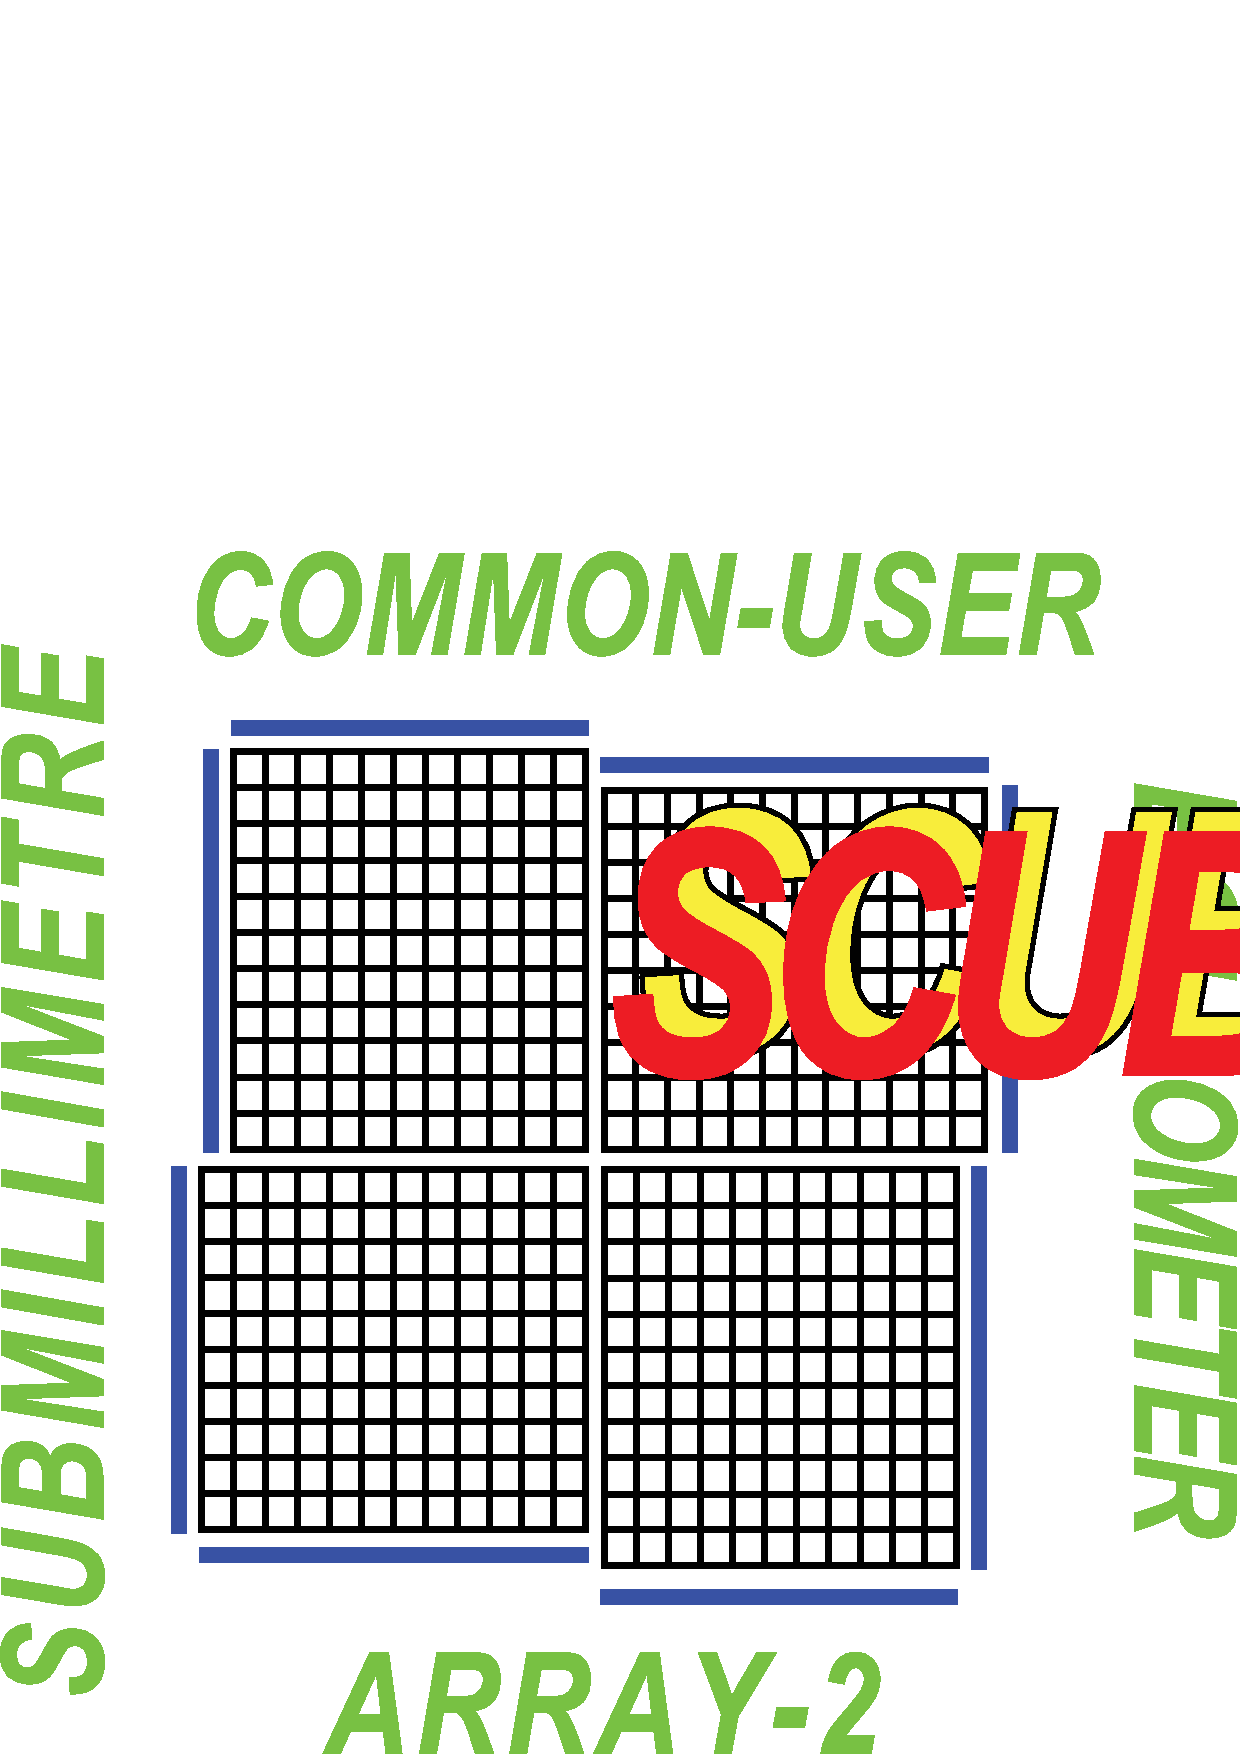
\includegraphics[scale=0.4]{s2logo}
\end{center}
 \vspace{5mm}
   \rule{\textwidth}{0.5mm}\\
   \vspace{5mm}
   \stardocauthors\\
  \vspace{10mm}
   \end{center}
   \vspace{5mm}

% ? Add picture here if required for the LaTeX version.
%   e.g. \includegraphics[scale=0.3]{filename.ps}

% ? End of picture

% ? Heading for abstract if used.
   \vspace{10mm}
   \begin{center}
      {\Large\textbf{Abstract}}
   \end{center}
% ? End of heading for abstract.
\end{latexonly}

%  HTML documentation header.
%  ==========================
\begin{htmlonly}
   \xlabel{}
   \begin{rawhtml} <H1> \end{rawhtml}
      %\stardoctitle\\
  %    \stardocversion\\
      \stardocmanual
   \begin{rawhtml} </H1> <HR> \end{rawhtml}

% ? Add picture here if required for the hypertext version.
%   e.g. \includegraphics[scale=0.7]{filename.ps}
\includegraphics[width=2.0in]{scuba_logo}
% ? End of picture

 \begin{rawhtml} <HR><hr> \end{rawhtml}

   \begin{rawhtml} <P> {\sl  \end{rawhtml}
   \stardoccategory\ \stardocnumber \\
   \stardocauthors \\
   \stardocdate

 \begin{rawhtml} <HR> \end{rawhtml}

   \begin{rawhtml} } </P> <H3> \end{rawhtml}
      \htmladdnormallink{University of British Columbia}
                        {http://www.ubc.ca} \\
      \htmladdnormallink{Science \& Technology Facilities Council}
                        {http://www.scitech.ac.uk} \\
   \begin{rawhtml} </H3> <H2> \end{rawhtml}
      \htmladdnormallink{Starlink Project}{http://www.starlink.ac.uk/}
   \begin{rawhtml} </H2> \end{rawhtml}
   \htmladdnormallink{\htmladdimg{source.gif} Retrieve hardcopy}
      {http://www.starlink.ac.uk/cgi-bin/hcserver?\stardocsource}\\

%  HTML document table of contents.
%  ================================
%  Add table of contents header and a navigation button to return to this
%  point in the document (this should always go before the abstract \section).
  \label{stardoccontents}

  \begin{rawhtml}
    <HR>
    <H2>Contents</H2>
  \end{rawhtml}
  \htmladdtonavigation{\htmlref{\htmladdimg{contents_motif.gif}}
        {stardoccontents}}

% ? New section for abstract if used.
\section{\xlabel{abstract}Abstract}
% ? End of new section for abstract
\end{htmlonly}

% -----------------------------------------------------------------------------
% ? Document Abstract. (if used)
%  ==================
\stardocabstract
% ? End of document abstract

% -----------------------------------------------------------------------------
% ? Latex Copyright Statement
%  =========================
\begin{latexonly}
\newpage
\vspace*{\fill}
\stardoccopyright
\end{latexonly}
% ? End of Latex copyright statement

% -----------------------------------------------------------------------------
% ? Latex document Table of Contents (if used).
%  ===========================================
  \newpage

  \begin{latexonly}

    \setlength{\parskip}{0mm}
    \tableofcontents
%\newpage
%\listoffigures
\thispagestyle{empty}
    \setlength{\parskip}{\medskipamount}
    \markboth{\stardocname}{\stardocname}
  \end{latexonly}
% ? End of Latex document table of contents
% -----------------------------------------------------------------------------

\cleardoublepage
\renewcommand{\thepage}{\arabic{page}}
\setcounter{page}{1}

\section{\xlabel{introduction}Introduction}
\label{sec:intro}

\subsection{\xlabel{using_guide}This Cookbook}

The Submillimetre Common User Bolometer Array-2 (SCUBA-2) is a
10,000-pixel bolometer camera for the 15-m James Clerk Maxwell
Telescope (JCMT). It has two arrays operating simultaneously to map
the sky in the atmospheric windows of 450 and 850\micron.

This guide is designed to instruct SCUBA-2 users on the best ways to
reduce and visualise their data using \starlink\ packages,
\smurf\cite{smurf}, \Kappa \cite{kappa}, \gaia \cite{gaia} and \picard
\cite{picard}.  This guide is {\em not} aimed at users of the
polarimeter (POL-2) or Fourier transform spectrometer (FTS-2). If you
have shared risk data (SRO) you should refer to the SMURF SRO
Cookbook\footnote{http://www.starlink.ac.uk/docs/sc19.htx/sc19.html}.

A brief description of the instrument and the observing modes is given
in Section~\ref{sec:s2}. Details on data acquisition and instructions
for examining raw data are given in Section~\ref{sec:raw}.
Section~\ref{sec:dimm} introduces the Dynamic Iterative Map-Maker
(DIMM). This section offers an in-depth description of the map-making
process and introduces the configuration files necessary to run the
reduction. The most important section will be Section~\ref{sec:maps};
this outlines all the steps that may be taken to produce your final
science map, including running the DIMM, applying the flux conversion
factor (FCF), co-adding multiple maps and estimating the noise. Section
\ref{sec:tweak} discusses your options for tweaking the configuration
parameters when running the map-maker; this gives you added control
and flexibility over the map-making routine. Two worked examples
covering different science case are shown in Section~\ref{sec:eg} -- a
blank cosmology field (\S\ref{sec:cosmology}) and a galactic field
(\S\ref{sec:bright_ex}) with bright, extended emission. Section
\ref{sec:pipe} introduces the science pipeline and data retrieval from
the JCMT Science Archive.  Data calibration is discussed in Section
\ref{sec:cal}, along with instructions for calculating your own FCF.

\subsection{\xlabel{computing}Before you start: Computing resources}

Before reducing SCUBA-2 data using the Dynamic Iterative Map-Maker, we
recommend you confirm your resources are sufficient for your type of
map.

For large-area maps it is important to process a full observation in a
single chunk -- see the text box on Page~\pageref{page:text} for a
discussion of the effects of chunking. For normal map-maker parameters
this implies that a machine of 96GB should be acceptable. It is
important that the memory is as fast as can be afforded as RAM speed
has a direct linear effect on processing time given that the
time-series data are continually being funneled through the CPU.  For
blank field surveys, data that only use 850 microns, or smaller
regions of the sky you can usefully run the map-maker with less memory
and 32 to 64GB is reasonable depending on the specifics of your data
set. SMURF is multi-threaded so multiple cores do help although above
8 cores the price/performance gains tend to drop off.

If you have a very large machine (128GB and 24 cores) you can to run
two instances of the map-maker in parallel. Use the SMURF\_THREADS
environment variable to restrict each map-maker to half the available
cores.

An alternative option is to download your reduced data from the JCMT
Science Archive at
CADC\footnote{http://www3.cadc-ccda.hia-iha.nrc-cnrc.gc.ca/jcmt/}. See
Section~\ref{sec:pipe} for details on the science pipeline and
retrieving your data from CADC.

\subsection{\xlabel{software}Before you start: Software}

This manual only uses software from the \starlink\ package;
\smurf\ \cite{smurf}, \Kappa\ \cite{kappa}, \gaia\ \cite{gaia} and
\picard\ \cite{picard}.
\starlink\ must be installed on your system, and \starlink\ aliases
and environment variables must be defined before attempting any
reduction of SCUBA-2 data detailed here. We also discuss the ORAC-DR
Data Reduction Pipeline\cite{oracdr} (hereafter just \oracdr) which is
an automated reduction pipeline, and \picard\ which is a similar
pipeline system for processing reduced data.

%For a more detailed description refer to the comprehensive Starlink User Note (\smurfsun)\footnote{currently SUN/258 is not completely up to date}.

%\textbf{\textsc{Smurf}} \textbf{and} \textbf{\textsc{Kappa}}\\*

The Sub-Millimetre User Reduction Facility, or \smurf, contains the
Dynamic Iterative Map-Maker (DIMM) that will process raw SCUBA-2 data
into images (see \smurfsun). \Kappa\ meanwhile is an application
package comprising general purpose commands for manipulating and
visualising NDF data (see \kappasun). Before starting any data
reduction you will want to initiate both \smurf\ and \Kappa.
\begin{myquote}
\begin{verbatim}
% smurf

        SMURF commands are now available -- (Version 1.4.0)

        Type smurfhelp for help on SMURF commands.
        Type 'showme sun258' to browse the hypertext documentation.
        Type 'showme sc21' to view the SCUBA-2 map-making cookbook.

% kappa

     KAPPA commands are now available -- (Version 1.13-9)

     Type kaphelp for help on KAPPA commands.
     Type 'showme sun95' to browse the hypertext documentation.

     See the 'Release Notes' section of SUN/95 for details of the
     changes made for this release.
\end{verbatim}
\end{myquote}
%\textbf{\textsc{Gaia}}\\*
Image visualisation can be done with \gaia\ (see \gaiasun). \gaia\ is an
image and data-cube display and analysis tool which incorporates tools such
as source detection, 3\textsc{d} visualisation, photometry and the ability
to query and overlay on-line or local catalogues.
\begin{myquote}
\begin{verbatim}
% gaia 850_map.sdf
\end{verbatim}
\end{myquote}

%\textbf{\textsc{Picard}}\\*
Post-processing analysis is performed using \picard. \picard\ documentation can be
found at \htmladdnormallinkfoot{the ORAC-DR web page}{http://www.oracdr.org/oracdr/PICARD},
or at \picardsun. All \picard\ recipes follow the same structure and are run like so:
\begin{myquote}
\begin{verbatim}
% picard -recpars <recipe_params_file> RECIPE <input_files>
\end{verbatim}
\end{myquote}
where \param{<recipe\_param\_file>} is a text file containing the
relevant recipe parameters, \param{RECIPE} is the name of the recipe
to be run (note the caps) and \param{<input\_files>} is a list of
files to be run, which must be int the current directory, or a
directory defined by \param{ORAC\_DATA\_OUT}. A number of \picard\
recipes will be demonstrated in Section~\ref{sec:maps}.

\textbf{Note:} The \picard\ recipes require all input files to have
the \texttt{.sdf} extension included; this is not the case for the
Starlink packages \Kappa\ and \smurf.

\clearpage
\section{\xlabel{scuba2_overview}SCUBA-2 Overview}
\subsection{\xlabel{scuba2}The instrument}
\label{sec:s2}

The SCUBA-2 bolometers are integrated arrays of superconducting
transition edge sensors (TESs) with a characteristic transition
temperature, $T_c$. In addition, each TES is ringed with a resistive
heater which can compensate for changes in sky power. The SCUBA-2
focal plane is kept at a base temperature slightly below $T_c$,
however a voltage is applied across each TES resistance to position
the bolometer at the transition temperature.  From this point, any
increase of temperature on the bolometers (e.g. from an astronomical
signal) will increase the TES resistance and heat it up. This causes a
drop in current and therefore a drop in temperature making the system
self-regulating.

For properly performing bolometers, the change in current through the
TES is proportional to the change in resistance, with the response
calibrated using flat-field observations (described below). This
changing current generates a magnetic field which is amplified by a
chain of superconducting quantum interference devices (SQUIDs). This
induces a feedback current which is proportional to the current
flowing through the TES, and it is this feedback current that is
recorded during data acquisition.

%Variation in T$_c$ across each subarray place maximum number of
%bolometer in the transition range.

Before science data can be taken the system must be optimised. These
`setups' are performed after slewing to the azimuth of the source,
where the SQUID, TES and heater biases are set to pre-determined
nominal values, in order to position the bolometers in the middle of
the transition range.

This is followed by a 10-second noise observation carried out while
the shutter is still closed. The shutter then opens onto the sky, and
as it does so the gradual increase in sky power hitting the array is
compensated for by a decrease in the resistive heater power via a
servo loop designed to keep the TES output constant. This acts to keep
the bolometers positioned at the centre of the transition range and is
known as \textbf{heater tracking}.

The responsivity of the bolometers will change slightly between the
dark and the sky; therefore, once the shutter is fully open a fast
\textbf{flat-field} observation is carried out to recalibrate them.
\textbf{A flat-field measures the responsivity of each bolometer to
changing sky power}. It does this by utilising the resistance heaters
which are ramped up and down around the nominal value. The change in
current through the TES is then recorded for each bolometer giving a
measure of its responsivity. The flat field solution is then the
inverse linear gradient of the current as a function of heater power.

At this point bolometers with responsivities above or below a
threshold limit are rejected, along with bolometers which display a
non-linear response or have a poor S/N.  A second flat-field is
performed at the end of an observation so bolometers whose
responsivity has changed over the course of the observation can be
flagged.

%Typically SCUBA-2 is referred to as having a field of view (FOV) of 8 square arcminutes. As you see in the image above the FOV is not quite square and as such a FOV a value of approximately 600\arcsec\ is more representative.

For full details of the array setup and operation see Holland et al.
(2012) \cite{s2main}.

\begin{figure}[t!]
\begin{center}
\includegraphics[width=0.4\linewidth]{450array.eps}
\hspace{1cm}
\includegraphics[width=0.4\linewidth]{850array.eps}
\label{fig:arrays}
\caption{\small The layout of the arrays at 450$\mu$m (left) and
850$\mu$m (right). The labels denote the name assigned to each
sub-array. Raw data files are generated separately for each sub-array
and must be co-added. This figure was made my running \wcsmosaic\ on
raw files from each sub-array.}
\end{center}
\end{figure}

\subsection{\xlabel{obs_modes}Observing modes}
\label{sec:mmodes}

Two observing modes are offered for SCUBA-2 -- \textsc{daisy} and
\textsc{pong}. As much of the work SCUBA-2 will be doing involves
large area mapping, both observing modes are scan patterns. Your
choice depends on the size of the area you wish to map, where you
would like your integration time concentrated and the degree of
extended emission you wish to recover

In contrast to SCUBA which observed an area of sky while
simultaneously chopping, SCUBA-2 removes atmospheric noise in the data
processing stage (Holland et al. 2012) \cite{s2main}. The power spectrum
of data taken by SCUBA-2 has a $1/f$ noise curve at lower frequencies. To
ensure astronomical signals are far away from this $1/f$ noise, fast
scanning speeds are required.

In order to disentangle source structure from other
slowly varying signals (e.g. extinction, sky noise, $1/f$ noise), the
scan pattern must pass across each region of the map from different
directions and at different times. The scan patterns themselves, along
with the associated parameters (velocity and scan-spacing), have been
designed and optimised to meet both these criteria.
\\*\\*
\begin{minipage}[t]{0.12\linewidth}
\textbf{PONG}
\end{minipage}
\begin{minipage}[t]{0.85\linewidth}\textsc{pong} maps are the scan
strategy for covering large areas. The default options allow for 3
sizes -- 900\arcsec, 1800\arcsec\ and 3600\arcsec. A single \textsc{pong} map is
a square of these dimensions and the telescope fills in the square by
bouncing off the edge of the area. To ensure an even sky background it
is recommended a minimum of 3, but preferably more than 5,
\textsc{pong} maps are included in a single observation with a
rotation introduced between each one. In this way a circular pattern
is built up, (see the right hand panel of Figure~\ref{fig:scan}), with
a diameter equal to your requested map size.
\vspace{0.2cm}\\
To recover large scale extended structure you are advised to use
larger \textsc{pong} maps which scan at a higher rate. This option is
in preference to tiling multiple smaller maps. Ultimately it is the
size of the SCUBA-2 field-of-view that determines the sensitivity to
large scale structure.
\end{minipage}
\\*\\*\\*
\begin{minipage}[t]{0.12\linewidth}
\textbf{DAISY}
\end{minipage}
\begin{minipage}[t]{0.85\linewidth}
\textsc{daisy} maps are the option for point-like or compact sources
($<$3\,arcmin) by maximising the exposure time on the centre of the
image. The telescope moves at a constant velocity in a `spirograph'
pattern that has the advantage of keeping the source on the array
throughout the observation. This is shown in the top panel of Figure
\ref{fig:scan}.
\end{minipage}


\begin{figure*}[b!]
\begin{center}
\includegraphics[width=0.9\linewidth]{wayne_scan.eps}
\caption{\small Telescope track in offsets of azimuth and elevation
for the SCUBA-2 observing patterns. \textbf{Top Left}: A single
rotation of the \textsc{daisy} pattern; \textbf{Top Right}: Multiple
rotations of the \textsc{daisy} pattern for a typical map based on a
180-arcsec demanded diameter; \textbf{Bottom Left}: A single
\textsc{pong} pattern; \textbf{Bottom Right}: Multiple rotations of
the \textsc{pong} pattern for a typical map based on an 1800\arcsec\
demanded map size. The scan pattern for your observation can be
visualised like this with \topcat\ using the output from \jcmtstate.
See Section~\ref{sec:exam} for more details. Figure taken from Holland
et al. (2012).}
\label{fig:scan}
\end{center}
\end{figure*}

\clearpage

\section{\xlabel{data_files}Raw SCUBA-2 Data}
\label{sec:raw}
A normal science observation will follow the following sequence.
\vspace{-2mm}
\begin{itemize}\itemsep-0.5em
\item Noise
\item Flat-field
\item Multiple Science scans
\item Flat-field
\end{itemize}
\vspace{-2mm}
The \param{SEQ\_TYPE} parameter in the fits header may be used to
identify the nature of each scan (see Section \ref{sec:fitsheader}).
When you access you data either at
the JCMT or by downloading from the Science
Archive\footnote{http://www3.cadc-ccda.hia-iha.nrc-cnrc.gc.ca/jcmt/}
you will get \emph{all} of the files listed above. Later when you
reduce your data using the map-maker you will include \emph{all} of
the files (noise + flat-fields + science).
Shown below is a list of the raw files for a single sub-array (in this
case s8a) for a short calibration observation. The first file is the
short, dark noise; the second and last scans are the fast flat-field
observations which occur after the shutter open to the sky at the
start of the observation and closes at the end (note the identical
file size); all of the scans in between are science. The SCUBA-2 data
acquisition (DA) system writes out a data file every 30 seconds; each
of which contains 23MB of data. The only exception is the final science
scan which will usually be smaller (7.3MB in the example below), typically
requiring less than 30 seconds of data to complete the observation.
\begin{myquote}
\begin{verbatim}
-rw-r--r-- 1 jcmtarch jcmt 6.2M Jul 19 21:33 s8a20120720_00030_0001.sdf
-rw-r--r-- 1 jcmtarch jcmt 9.6M Jul 19 21:34 s8a20120720_00030_0002.sdf
-rw-r--r-- 1 jcmtarch jcmt  23M Jul 19 21:34 s8a20120720_00030_0003.sdf
-rw-r--r-- 1 jcmtarch jcmt  23M Jul 19 21:35 s8a20120720_00030_0004.sdf
-rw-r--r-- 1 jcmtarch jcmt  23M Jul 19 21:36 s8a20120720_00030_0005.sdf
-rw-r--r-- 1 jcmtarch jcmt  23M Jul 19 21:36 s8a20120720_00030_0006.sdf
-rw-r--r-- 1 jcmtarch jcmt 7.3M Jul 19 21:36 s8a20120720_00030_0007.sdf
-rw-r--r-- 1 jcmtarch jcmt 9.6M Jul 19 21:37 s8a20120720_00030_0008.sdf
\end{verbatim}
\end{myquote}
\textbf{Note:} All of these files are written out 8 times for each of the
8 sub-arrays.

The main data arrays of each file are cubes, with the first two
dimensions enumerating columns and rows, and the third time slices
(sampled at 200\,Hz).

Raw SCUBA-2 data comes in uncalibrated units. The first calibration
step is to scale the raw data to units proportional to picowatts (pW)
by applying the flat-field solution. From there the data must be
scaled by the flux conversion factor (FCF) to give units of Janskys
(Jy).

The first step is applied internally by the map-maker but can be done
manually when examining the raw data -- see Section \ref{sec:concat}.
The second step must be done manually with instructions are given in
Section~\ref{sec:cmult}.


\subsection{\xlabel{examine}Examining raw data}
\label{sec:exam}

In this section a number of procedures are described for visualising
and assessing raw data files.  These steps are not a necessary part of
the data reduction process and do not concern the iterative map-maker.
However, there are reason you may wish to do examine your raw data in
greater depth. The most likely motivation is unusual result from the
map-maker. These might be higher noise than anticipated, patterns in
the data or inconsistent noise across multiple tiles. This section
will help you get to the bottom of any issues concerning raw data.

\subsubsection{\xlabel{concat}Concatenate \& apply a flat-field}
\label{sec:concat}

Since SCUBA-2 data for a given sub-array are broken into multiple
30\,second scans by the data acquisition (DA) system, it is useful to
concatenate the data into a single file. The \smurf\ task \concat\ can
be used for this operation. The example below combines all of the
files associated with observation 8 for the s8a array into a single
file called \texttt{s8a20120725\_00058\_con}.

\begin{myquote}
\begin{verbatim}
% sc2concat 's8a20120725_0008*.sdf' s8a20120725_0008_con
\end{verbatim}
\end{myquote}
\concat\ will automatically filter out any dark or flat-field
observations, so that the concatenated file contains only the science
data. Be careful when concatenating a very long observation since the
output file may be too large to reasonably handle. Fifteen minute
chunks (30 files) should be sufficient.

\concat\ applies the flat-field by default (although it can be
disabled using the `noflat' option on the command-line).

The flat-field can also be applied manually using the \flatfield\ command.

\begin{myquote}
\begin{verbatim}
% flatfield 's8a20120701_0008*.sdf' '*_flat'
\end{verbatim}
\end{myquote}
Here, the output will be a flat-fielded version of each science scan
in observation number 8; the file names will be the original input
names with \_flat appended to them.

As a rule of thumb, you should apply the flat-field to your data
before examining it. \textbf{You do not need to apply the flat-field
prior to reducing your data with the map-maker as it will be applied
internally.}



\subsubsection{\xlabel{header}Headers and file structure}
\label{sec:fitsheader}
There are two \Kappa\ tasks which are extremely useful for examining
your data: \fitslist\ and \ndftrace, which can be used to view the
FITS headers and dimensions of the data.
\\*\\*
\begin{minipage}[t]{0.12\linewidth}
\textbf{fitslist}
\end{minipage}
\begin{minipage}[t]{0.85\linewidth}This lists the fits header information
for any file (raw or reduced). This extensive list includes dates \& times,
source name, scan type, pattern and velocity, size of the map, exposure
time, start and end elevation, opacity and the temperature of the
instrument. An example is given below:
\begin{myquote}
\begin{verbatim}
% fitslist s8a20120720_00030_000\*.sdf | grep SEQ_TYPE
\end{verbatim}
\end{myquote}
If you already know the name of the parameter you want to view you can
use the \fitsval\ command instead, e.g.
\texttt{\% fitsval file.sdf TAU225ST}.\\*
\end{minipage}

\begin{minipage}[t]{0.12\linewidth}
\textbf{ndftrace}
\end{minipage}
\begin{minipage}[t]{0.85\linewidth}
\ndftrace\ displays the attributes of the data structure. This will tell
you the units of the data, pixel bounds, dimensions and axis assignations.\\*
\end{minipage}
\\*\\*
Full details of these commands can be found in the \xref{\Kappa\ manual}{sun95}{}.


\begin{figure}[ht!]
\begin{center}
\begin{fmpage}{0.95\linewidth}
\vspace{0.2cm}
\textbf{ Topcat Example}

\vspace{0.5cm}

\begin{minipage}[c]{0.6\linewidth}

\begin{myquote}
\begin{verbatim}
% topcat -f tst 20120720_30.tst
\end{verbatim}
\end{myquote}
\end{minipage}
\hspace{0.3cm}
\begin{minipage}[c]{0.32\linewidth}
Load the file into \topcat\ with this command.
\end{minipage}

\vspace{0.5cm}

\begin{minipage}[c]{0.6\linewidth}
\centering
\includegraphics[width=0.95\textwidth]{topcat1.eps}

\end{minipage}
\hspace{0.3cm}
\begin{minipage}[c]{0.32\linewidth}
Once the file has loaded into \topcat, select the scatter plot option
from the menu bar across the top of the window.
\end{minipage}

\vspace{0.5cm}

\begin{minipage}[c]{0.6\linewidth}
\centering
\includegraphics[width=0.75\textwidth]{topcat2.eps}
\vspace{0.2cm}
\end{minipage}
\hspace{0.3cm}
\begin{minipage}[c]{0.32\linewidth}
When the scatter plot has loaded, you should adjust the $X$-axis and
$Y$-axis values to DRA and DDEC respectively to display the scan pattern.
If you are interested in seeing how any of the variables change over time,
select the the $X$ Axis to be either Id or RTS\_NUM.
\end{minipage}

\end{fmpage}
\end{center}
\caption{\small \topcat\ example demonstrating how to display the scan pattern
for an observation.}
\label{fig:topcat}
\end{figure}


\subsubsection{\xlabel{scan_pat}Displaying scan patterns}
\label{sec:scan}

The movement of the telescope throughout a scan (as well as other
state information) is stored in the \texttt{MORE.SMURF.JCMTSTATE}
extension of a data file. The \smurf\ task \jcmtstate\ converts this
information into a simple ASCII tab-separated table.

\begin{myquote}
\begin{verbatim}
% jcmtstate2cat s8a20120701_00008_*.sdf > state.tst
\end{verbatim}
\end{myquote}

The `-h' option to \jcmtstate\ can be used to find more information on
the command. In particular, multiple files can be supplied to the
command using standard shell wild cards. If you have already
concatenated your data you can simply input the single concatenated
file. \textbf{It may be useful to view the scan pattern for your
observation, particularly for maps taken at high elevations, to ensure
the pattern completed successfully.}

% (not escaped) and for SCUBA-2 data the `--with-mce' option can be used to dump the low-level MCE header information.

This catalogue can be loaded into \topcat\ for plotting, making sure
to specify the TST format during loading.

\begin{myquote}
\begin{verbatim}
% topcat -f tst state.tst
\end{verbatim}
\end{myquote}

Example of scan patterns displayed with \topcat\ can be seen in
Figure~\ref{fig:scan}. Detailed instruction on how to display the scan
pattern for your observation are given in Figure~\ref{fig:topcat}. All
of the time-varying header values are available for plotting.  Other
values include the azimuth and elevation offsets (DAZ \& DEL), the WVM
and 225\,GHz opacity values and the instrument temperatures (e.g.
SC2\_FPUTEMP gives the temperature of the focal plane).

Due to extreme accelerations at ``turn-around'' points of a scan
pattern (especially for \textsc{pong}s), the telescope finds it hard
to follow the proscribed scan patterns at high elevations. To mitigate
this we try to avoid observing any sources above 70$^\circ$ elevation.
If the \fitslist\ parameters \param{ELSTART} and \param{ELEND}
indicate that your map was taken at high elevation you may consider
checking the success of the scan pattern. If you find your observation
has failed to follow the demanded scan pattern don't worry, the data is
likely to still be useful. This is especially true for \textsc{daisy}
maps where the high exposure-time central region is usually
unaffected.

\subsubsection{\xlabel{display_cube}Displaying time-series data}
\label{sec:gaiacube}

%\vspace{-2mm}
%\begin{itemize}
%\item \emph{Examine each bolometer to check the stability}
%\end{itemize}
%\vspace{-3mm}
\begin{figure}[h!]
\includegraphics[width=\linewidth]{gaia1.eps}
\vspace{1mm}
\caption{\small Initial \gaia\ windows displayed upon loading a data cube.
  The main window in the left shows a map of bolometer values at a fixed
  sample in time. You may have to zoom in multiple times by clicking the
  `Z' icon. On the right-hand side, the `Display image sections of a cube'
  dialogue enables the user to navigate the time axis.}
\label{fig:gaia_main}
\end{figure}

\begin{figure}[h!]
\centering
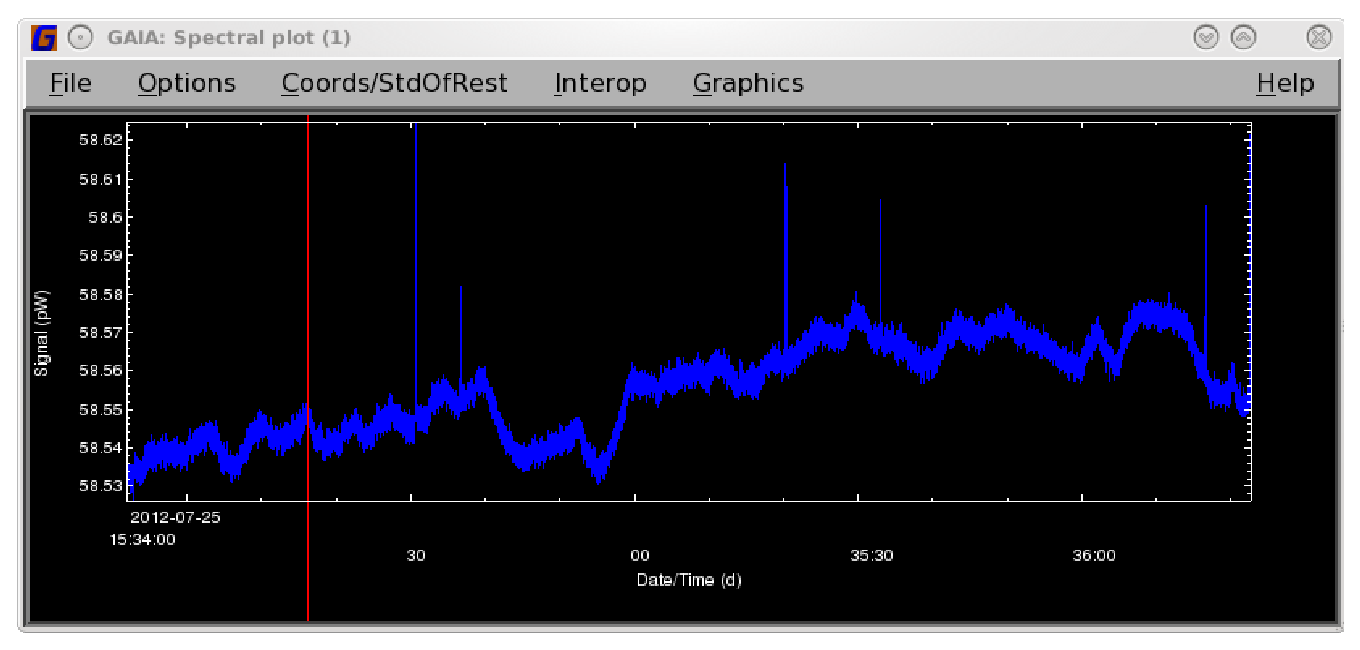
\includegraphics[width=0.8\linewidth]{gaia2.eps}
\vspace{0.3cm}
\caption{\small The \emph{Spectral Plot} window displaying its time-varying
signal, appears automatically once a bolometer is clicked in the main window.
The vertical red line indicates the time slice that is currently selected
in the `Display image sections of a cube' dialogue -- this can be dragged
across the spectrum to scroll through the time-slices.}
\label{fig:gaia_spec}
\end{figure}

Use the \starlink\ application \gaia\ to visualise the bolometer time
series data (or indeed \emph{any} SCUBA-2 data file). This is
initiated simply typing \texttt{gaia} into a terminal.

\begin{myquote}
\begin{verbatim}
% gaia s8a20120725_00058_con.sdf
\end{verbatim}
\end{myquote}

Loading a file in \gaia\ produces two windows (see
Figure~\ref{fig:gaia_main}). The main window shows a map of bolometer
values at a given point in time. The time slice displayed may be
changed by scrolling through the time axis. This is done in the second
window entitled `Display image sections of a cube'. The `Index of
plane' slider towards the top of this window may be moved to display
different time slices in the main window.

A third window will appear when you click on a bolometer -- the
`Spectral plot'. This shows an automatically scaled plot of the raw
time stream of data for that given bolometer. It will be overridden
when you click on a different bolometer.

A second way to scroll through the time axis is to click and drag the
vertical red bar on the `Spectral plot' window. As you do so array
shown in the main window will automatically update.

To highlight small variations between bolometers it is likely you will
need to change the auto cut and (depending on your preference) the
colour scheme -- both are controlled by buttons on the sidebar.

See the \xref{\gaia\ manual}{sun214}{} for full
details.\footnote{http://docs.jach.hawaii.edu/star/sun214.htx/sun214.html}

\clearpage
\subsection{\xlabel{regrid_map}Regridding data into a map}
\label{sec:regrid}

Any raw time-series data can be quickly regridded into sky frame
coordinates using the \smurf\ \makemap\ task in regrid mode. This
involves no processing of the data. The following command produces a
map from the raw concatenated data; unlike the iterative mode of
\makemap\ described in the next chapter, no configuration file is
required.
\begin{myquote}
\begin{verbatim}
% makemap s8a20120725_00058_con.sdf crl2688_sky method=rebin
\end{verbatim}
\end{myquote}
The output map here is called `\texttt{crl2688\_sky.sdf}' and is shown
in Figure~\ref{fig:regrid}.
The pixel scale is left at the default values of 2~arcsec on a side at
450\micron\ and 4~arcsec at 850\micron\ (although this can be changed
using the `pixsize=$x$' option on the command-line, where $x$ is in
arcsec).

\subsection{\xlabel{clean}Notes on cleaning your data}
\label{sec:clean}
Cleaning raw data is an essential first step towards making a quality
final map. The map-maker performs all of these cleaning steps during
the pre-processing stage. The commands for manually cleaning your data
are given in Appendix~\ref{app:clean}.

You can also check out the SMURF SRO
Cookbook\footnote{http://www.starlink.ac.uk/docs/sc19.htx/sc19.html}
which goes into great depth on the data cleaning options.
\begin{figure}[b!]
\begin{center}
\includegraphics[width=0.65\linewidth]{crl2688_regrid.eps}
\caption{\small The regridded map of CRL2688 with the s8a sub-array displayed with \gaia.}
\label{fig:regrid}
\end{center}
\end{figure}


\subsection{\xlabel{calcnoise}Checking the array performance}
\label{sec:calcnoise}

The on-sky performance of the array can be assessed using the \smurf\
command \calcnoise. Rather than give an absolute measure, \calcnoise\
should be used as an indicator of array performance and stability.
\calcnoise\ cleans the data then calculates the
white noise on the array (between 2 and 10\,Hz by default). If the
dark noise scans are given as input, this will track the array
sensitivity independent of sky conditions. If you provide the whole
observation (as in the example below) then the dark files will be
ignored and the on-sky performance of the array is calculated.

\begin{myquote}
\begin{verbatim}
% calcnoise s8a20110720_00030*.sdf s8a_noise method=! power=!
\end{verbatim}
\end{myquote}
It will prompt for a configuration file to describe the cleaning
steps -- the default is the supplied \texttt{dimmconfig\_calcnoise.lis}.
Two noise measurements are reported in the terminal: the
`Effective noise' and the `Effective NEP'.

An output file is created for each sub-array with the NEP map stored
in the \texttt{.MORE.SMURF.NEP} extension.

If you have a bright source in the field this will
contaminate the signal. In this case you should examine the
\texttt{NOI} model from the map-maker instead -- see Section
\ref{sec:models} for a description and Section~\ref{sec:export} for
details on how to examine it.
%\raggedbottom

\clearpage
\section{\xlabel{dimm}The Dynamic Iterative Map-Maker}
\label{sec:dimm}

The Dynamic Iterative Map-Maker (DIMM), hereafter just referred to the
the map-maker is the tool you will use to produce SCUBA-2 maps. It
performs all pre-processing steps to clean the data, followed by
iteratively solving for multiple signal components and regridding to
produce a final science map.

This section describes the process by which the map-maker reduces
data. It is essential reading to gain an understanding of what has
happened to produce your reduced image, especially if you wish to
modify the default map-maker parameters. Nevertheless, this is manual
is intended to present `need to know' information for data reduction.
For full details of the map-maker see \textbf{Chapin et al. (2012)} \cite{mapmaker}.

\subsection{\xlabel{dimm_theory}The theory}

The map-maker works by individually modelling the various
contributions that make up the signal recorded by each bolometer. It
models and then subtracts all the sources of signal in order of
decreasing magnitude, ultimately leaving just the astronomical signal
plus noise. A list of the modelled components can be seen in Table
\ref{tab:mods} and a description found in Section~\ref{sec:models}.

The map-maker requires a configuration file to accompany each
reduction. This file instructs the map-maker on the pre-processing
steps, which components to iteratively model, the parameters to use
when doing so, and finally the stopping (or convergence) criteria.
There is single `master' configuration file -- \texttt{dimmconfig.lis}
-- which contains \emph{all} the available options (though most are
commented out by default) and is fully documented. A copy of this file
is available in Appendix~\ref{app:dimm}.

Often, the default configuration file will not give optimal results
for your particular observation. For this reason, specialised
configuration files have been developed which are tailored to
different science goals, be they detecting faint galaxies or mapping
large molecular clouds. Neevertheless, these specialised models A
description of these specialised configuration files can be found in
Section~\ref{sec:config}.
\\*\\*
{\large{\texttt{\bf dimmconfig.lis}}}\\*
Figure~\ref{fig:dimm} shows of flow chart of the map making process
for \texttt{dimmconfig.lis}. It is divided into two sections: the
pre-processing stage where the data are cleaned, then the iterative
stage where the different models are subtracted.
Table~\ref{tab:dimmdef} gives all the variables in
\texttt{dimmconfig.lis} again divided into the two main stages.

The first task the map-maker perform is to down-sample the data. The
raw time-series data is re-sampled at a rate that matches the
requested pixel size, the equivalent to applying a low-pass filter.
Down-sampling saves time and memory usage when running the map-maker.
The raw data is then concatenated and has the flat-field (from the
bracketing fast flat scans) applied to calibrate the bolometers. A
number of cleaning steps are then run: a polynomial baseline is
subtracted from each bolometer; spikes and dc steps are removed; any
resulting gaps in the time-series are filled in.

Next comes the iterative stage of the process. First to be modelled
and removed are \texttt{COM} and \texttt{GAI} which work together to
calculate the average signal template of all the bolometers, and then
fit/remove the templates from each bolometer. The next model
(\texttt{EXT}) applies a multiplicative extinction correction to the
data.  Following this, a Fourier transform is applied to the data and
the \texttt{FLT} model is removed in the frequency domain.
\texttt{FLT} applies a high-pass filter to the data, above frequencies
that correspond to angular scales of 600\,arcsec and 300\,arcsec at
450\micron\ and 850\micron, respectively.

Next comes the \texttt{AST} model, the first step of which involves
regridding the data to produce an estimation of the final science map.
Since many samples typically contribute to the estimate of the signal
in a given pixel, the noise is greatly reduced compared with the
time-series data. This map is then projected back into the time series
and the \texttt{AST} model removed. The \texttt{NOI} model then
measures the noise in the residual signals for each bolometer to
establish weights for the data as they are placed into the map in
subsequent iterations.

At this stage convergence is checked against the parameters detailed
in the configuration file.  Convergence is achieved either when the
requested number of iterations has been completed or when the
noise-based convergence criteria specified in the configuration file
is reached. If more iterations are required or (in the latter case)
the residual noise has not converged then \texttt{GAI}, \texttt{EXT},
\texttt{FLT} and \texttt{COM} models are all un-done and the
time-series is reconstructed. The sequence is then re-run only this
time without \texttt{AST} complicating the model fitting.

\begin{figure}
\begin{center}
\includegraphics[width=0.78\linewidth]{flow_dimm_blue.eps}
\caption{\small A flow chart illustrating the dynamic iterative map-maker.
Note that for each iteration the \texttt{AST} model is subtracted from
the time-series leaving only those contributions to be fitted and removed.}
\label{fig:dimm}
\end{center}
\end{figure}


\setlength{\extrarowheight}{3pt}
\begin{table}
\centering
\begin{tabular}{c|l}
\hline
\textbf{Model} &\hspace{0.2cm} \textbf{Description} \\
\hline
\texttt{COM}&\hspace{0.2cm} Common-mode signal\\
\texttt{GAI}&\hspace{0.2cm} Common-mode scaled to each bolometer -- the gain\\
\texttt{EXT}&\hspace{0.2cm} Extinction correction\\
\texttt{FLT}&\hspace{0.2cm} Fourier transform filter\\
\texttt{AST}&\hspace{0.2cm} Map estimate of astronomical signal\\
\texttt{NOI}&\hspace{0.2cm} Noise estimation\\
%\hline
%\texttt{DKS}&\hspace{0.2cm} Dark squid cleaning along columns\\
%\texttt{PLN}&\hspace{0.2cm} 2-dimensional time-varying plane removal\\
%\texttt{SMO}&\hspace{0.2cm} Time domain smoothing filter\\
%\texttt{TMP}&\hspace{0.2cm} Pointing ans baseline template\\
\hline
\end{tabular}
\label{tab:mods}
\caption{\small Table adopted from Chapin et al. (2012). A fuller
explanation of each model is given below.}
\end{table}

\raggedbottom
\subsection{\xlabel{models}The individual models}
\label{sec:models}

The particular sequence of the models evaluated (and removed) by the
map-maker during the iterative stage is indicated by the
\texttt{modelorder} parameter in the configuration file. These models
are modular however so their order may be changed. The default model
order in \texttt{dimmconfig.lis} is given below.
\vspace{-0.1cm}
\begin{myquote}
\begin{verbatim}
modelorder = (com,gai,ext,flt,ast,noi)
\end{verbatim}
\end{myquote}
\vspace{-0.1cm}
The only recipe not following this model order is the one tailored for
blank field maps which does not include a \texttt{FLT} model in the
iterative stage (see Section~\ref{sec:config}). Below is a basic
description of each model, while more complete descriptions of the
models and all the associated caveats can be found in Chapin et al.
(2012) \cite{mapmaker}.
\\*\\*
\begin{minipage}[t]{0.07\linewidth}
\texttt{COM}
\end{minipage}
\begin{minipage}[t]{0.92\linewidth}The \texttt{COM} model removes the
common-mode signal (the signal that is common to all bolometers), the
dominant contributor to this signal being the sky noise. It determines
this by simply averaging over all bolometers for each time slice.
Bolometers are flagged as bad, (and thus omitted from the final map), if
they do not resemble the \texttt{COM} model seen by the majority of the
other bolometers.
\newline Extended emission on a scale larger than the array footprint
on the sky will contribute a signal indistinguishable from a
common-mode signal. This puts an upper limit on the spatial scale of
astronomical emission that can be recovered. \\*
\end{minipage}

\begin{minipage}[t]{0.07\linewidth}
\texttt{GAI}
\end{minipage}
\begin{minipage}[t]{0.92\linewidth}The \texttt{GAI} model works with
\texttt{COM} in removing the common-mode signal. \texttt{GAI} is used to
scale the \texttt{COM} model that has been subtracted and is described by
a gain and an offset to scale all the bolometers to the same level. This
will allow the bolometers to share a common calibration further down the
line. \\*
\end{minipage}
\begin{minipage}[t]{0.07\linewidth}
\texttt{EXT}
\end{minipage}
\begin{minipage}[t]{0.92\linewidth}\texttt{EXT} applies the extinction
correction. This is a time-varying scaling factor that is derived from
the JCMT water vapour radiometer. As it deals with 30-second chunks of
data this accounts for varying conditions over a long observation. For
more details see Section~\ref{sec:cal}. \\*
\end{minipage}
\begin{minipage}[t]{0.07\linewidth}
\texttt{FLT}
\end{minipage}
\begin{minipage}[t]{0.92\linewidth}The \texttt{GAI} model acts on the FFT
of the bolometer data. High-pass (only allows \emph{higher} frequencies to
pass) and low-pass (only allows \emph{lower} frequencies to pass) filters
can be specified. These cut-off frequencies can either be be specified by
the user directly or as an angular spatial scale (which is subsequently
converted into a frequency dependent on the speed at which the
telescope is moving). The most important role of this model is to
apply a high-pass filter in order to remove the $1/f$ noise. Note that
extended emission varies slowly over the array; it therefore appears
at low frequencies and complicates the choice of a high-pass filter. A
further discussion of this matter is given in
Section~\ref{sec:bright_ex}\\*
\end{minipage}
\begin{minipage}[t]{0.07\linewidth}
\texttt{AST}
\end{minipage}
\begin{minipage}[t]{0.92\linewidth}This step involves both the creation of the
\texttt{AST} model and the final science map. Hence, the position of
\texttt{AST} in the model order indicates at what stage the astronomical
image should be estimated. When the \texttt{AST} model is called, the first
step is regridding the raw time-series data, (using nearest-neighbour sampling),
to produce an estimate of the final map. Following this, the map is
projected back into the time domain and removed (as the \texttt{AST}
model).\\*
\end{minipage}
\begin{minipage}[t]{0.07\linewidth}
\texttt{NOI}
\end{minipage}
\begin{minipage}[t]{0.92\linewidth}\texttt{NOI} should come last in the model
order and calculates the RMS noise in each bolometer.  \texttt{NOI} is
determined by running \calcnoise\ (see Section~\ref{sec:calcnoise}) on
the residual signal (the \texttt{RES} model, see
Section~\ref{sec:export}).  Unlike the other models, \texttt{NOI} is
not a subtraction or a correction but if specified, is used (from the
second iteration onwards) to weight the bolometers in the map
estimate.
\end{minipage}

\subsection{\xlabel{convergence}Convergence}
\label{sec:converge}

The convergence criteria is crucial to the success of the iterative
process. Convergence is achieved when the requested number of
iterations has been completed \textbf{OR} when the convergence
criteria specified in the configuration file is reached.

Specifying the number of iterations in the configuration file is done via
the \texttt{numiter} parameter. In \texttt{dimmconfig.lis}, this is given
by:
\vspace{-0.1cm}
\begin{myquote}
\begin{verbatim}
numiter = -5
\end{verbatim}
\end{myquote}
\vspace{-0.2cm}
A positive value for \texttt{numiter} means that the requested number
of iterations will be executed. A negative value, as in the example
above, indicates that no more than this number of iterations should be
performed, \emph{but} that it may stop at fewer if convergence
(according to the noise criteria below) has been achieved.

There are two parameters in the configuration file for specifying a
convergence criteria based on noise:
\\*\\*
\begin{minipage}[t]{0.1\linewidth}
\texttt{chitol}
\end{minipage}
\begin{minipage}[t]{0.9\linewidth}This test checks the change in the
reduced chi-squared, $\chi^2$, with the standard deviations being
measured for each of the residual bolometers signals once all the
model components have been removed. Note that it is the noise in the
time-series data that is being checked. The map has converged once the
the change is consecutive values of $\chi^2$ is less than the
parameter \texttt{chitol}.
\end{minipage}
\vspace{2mm}

\begin{minipage}[t]{0.1\linewidth}
\texttt{maptol}
\end{minipage}
\begin{minipage}[t]{0.9\linewidth}
This is the average normalised change in the value of map pixels
between subsequent iterations. Convergence is reached when the change
is less than the parameter \texttt{maptol}. It has units of the noise
in the map, thus \texttt{maptol}$=$0.05 means a change of
$<$0.05\,$\sigma$. This option has the advantage of directly assessing
the noise in the resulting map rather than the time-series.
\vspace{3mm}\\
Typically the normalized change in pixel values between iterations
drops rapidly to begin with and then flattens out, decreasing
increasingly slowly. As a result, in some circumstances, the map-maker
will fail to stop iterating due to low frequency ripples coming and
going between iterations.
\vspace{3mm}\\
\texttt{maptol} is the default for those recipes which use
masking -- \texttt{dimmconfig\_bright\_extended.lis} and
\texttt{dimmconfig\_bright\_compact.lis} -- where other constraints
ensure the map converges. There is limited use in setting
\texttt{maptol} to lower than 0.05  as it will dramatically increase
the length of time to produce the final map, possibly never converging,
yet with marginal improvement.
\vspace{3mm}\\
\end{minipage}
The best way of checking the progress of convergence while running the
map-maker is to use the \param{itermap} option and setting
\param{itermap = 1} (see Section~\ref{sec:tweak}).

\begin{figure}
\begin{center}
\includegraphics[width=\linewidth]{com.eps} \\
\includegraphics[width=\linewidth]{flt.eps} \\
\includegraphics[width=\linewidth]{ast.eps} \\
\includegraphics[width=\linewidth]{res.eps} \\
\caption{Time-domain components of the iterative models. These show the
solution for the same single bolometer for part of an observation of
CRL2688. From top to bottom: the \texttt{COM} model containing signal
common to all bolometers, the \texttt{FLT} model containing residual
low-frequency noise missed by \texttt{COM}, the \texttt{AST} model
with the signal showing as a positive spike when this bolometer passes
over the source, and the \texttt{RES} model looking (as expected) like
white noise. }
\label{fig:itercomp}
\end{center}
\end{figure}



\subsection{\xlabel{export}Exporting individual models}
\label{sec:export}

By default, the final values of these fitted models are {\em not}
written out to files. However, this can be changed by setting
\texttt{exportndf} in the configuration file to the list of models
that you wish to view.

You can an additional component, \texttt{RES}, if you wish to export
the residual model. \texttt{RES} is the residual signal remaining
after the other models have been removed. By contrast, the
\texttt{NOI} model is the noise in \texttt{RES}, as determined by
running \texttt{RES} through \calcnoise\ (see
Section~\ref{sec:calcnoise}). If \texttt{NOI} is exported, it can be
viewed as the VARIANCE component of the \texttt{RES} model; thus,
export of \texttt{RES} is implied if \texttt{NOI} is specified.
%QUA It tells you which bit of each bolometer time-series has been flagged and the value is the reason for flagging. is specified, as it becomes the variance component of the resulting NDF for \texttt{RES}. \texttt{QUA} will become the quality component of any full 3-dimensional model (i.e. \texttt{RES}, \texttt{AST}, \texttt{FLT}, \texttt{EXT}).

\vspace{0cm}
\begin{myquote}
\begin{verbatim}
exportndf = (com,gai,ast,flt,res,noi,qua)
\end{verbatim}
\end{myquote}
\vspace{0cm}
The \texttt{exportndf} parameter will write out the requested models
as NDF files with names based on the first input file that went into
the maps for each sub-array. This is first suffixed by `\texttt{con}',
indicating that several data files may have been concatenated
together. The filename is then appended by the 3-letter code for each model (such as
\texttt{s8a20120720\_00030\_0003\_con\_com.sdf},
\linebreak
\texttt{s8a20120720\_00030\_0003\_con\_flt.sdf},
\texttt{s8a20120720\_00030\_0003\_con\_res.sdf})\footnote{The filename shows
sub-scan 3 of Observation 30 since this is the first science file that
is encountered (see Section~\ref{sec:raw}.}. The variance
and quality for the data are stored as the VARIANCE and QUALITY
components within the residual file NDF.

As with the input data, these are all standard \starlink\ NDF files
which can be examined using all of the existing \starlink\ tools.

Examples of the time traces for a single bolometer from these output
models is shown in Figure~\ref{fig:itercomp}.  These traces cover a
subset of an observation of the secondary calibrator CRL2688. The
\texttt{COM} model is removed first, being the dominant source. The
\texttt{FLT} model stores the data removed by the high-pass filter. In
the \texttt{AST} model, CRL2688 is clearly seen as positive spikes
which appear when the bolometer passes over the source. Finally, the
residual signal stored in \texttt{RES} is flat, indicating that most
of the signal has been successfully accounted for by the other model
components.


\renewcommand*\arraystretch{0.85}
\begin{table*}
\begin{center}
\begin{footnotesize}
\begin{tabular}{|p{2.2cm}|p{1.1cm}|p{11.4cm}|}
\hline
Param & Value & Description \\
\hline
\multicolumn{3}{|l|}{\textbf{General}}\\
\hline
numiter       &   -5 & Number of iterations. A negative number = max iterations
                       if using $\chi^2$ and/or map stopping criteria\\
chitol        & 1e-3 & Threshold change in reduced $\chi^2$ in subsequent
                       iterations.\\
varmapmethod  &    1 & Estimate variance map by sample variance of data that
                       land in each pixel\\
maxlen        &    0 & Maximum length (secs) for concatenated data. 0 = attempt
                       to concatenate entire chunks\\
exportndf     &    0 & Do not export any models\\
downsampscale &   -1 & Down-sample to save memory and time. Negative value = its
                       magnitude will be multiplied by the PIXSIZE for the
                       requested map.\\
\hline
\multicolumn{3}{|l|}{\textbf{Pre-Prcoessing}}\\
\hline
order         &    1  & Subtract a baseline polynomial of this order\\
apod          & undef & Use default apodisation based on filter frequency\\
badfrac       & 0.05  & Fraction of samples to be bad to flag entire bolometer
                        as dead\\
flagslow      &    30 & Flag data taken while telescope was moving so slowly
                        that sources sit in $1/f$ noise\\
450.flagfast  &  1000 & \multirow{2}{*}{{\large$\rbrace$}\,Flag data taken
                        the telescope was moving too fast causing source
                        smearing}\\
850.flagfast  &  1000 & \\
pcathresh     &     0 & PCA cleaning is the threshold above which components
                        will be removed from the bolometer time-series.\\
dcthresh      &  25.0 & S/N threshold to detect DC step\\
dcfitbox      &    30 & Box size over which to fit data with a straight
                        line on either side of a potential DC jump\\
dcmaxsteps    &    10 & The maximum number of steps that can be corrected
                        in each minute of good data.\\
dclimcorr     &     0 & If more than DCLIMCORR bolometer have a step at
                        a given time, then all bolometers are corrected for
                        a step at that time, using lower thresholds.\\
dcsmooth      &    50 & The width of the median filter used to smooth a
                        bolometer data stream prior to finding DC jump\\
fillgaps      &     1 & Fill vicinity of spikes/DC steps with constrained
                        realization of noise\\
noisecliphigh &   4.0 & Clip bolometers based on their noise. This step
                        will remove any bolometers noisier than noisecliphigh
                        standard deviations above the median.\\
\hline
\multicolumn{3}{|l|}{\textbf{Iterative}}\\
\hline
com.oldalg       &    0 & Set this flag to a non-zero value to use the old COM
                          algorithm. Not recommended.\\
com.niter        &    1 & The number of n-sigma clipping iterations (1 = no clipping)\\
com.nsigma       &    3 & The number of standard deviations at which the 3\,$\sigma$
                           clipping algorithm clips\\
com.noflag       &    0 & If set, disable flagging of bad bolos using common-mode.\\
com.corr\_tol    &    5 & $n$-sigma away from mean correlation coefficient tolerance\\
com.gain\_tol    &    5 & $n$-sigma away from mean gain coefficient tolerance\\
com.gain\_abstol &    3 & Absolute factor away from mean gain coefficient tolerance\\
com.gain\_box    &-30.0 & The number of time slices (or seconds if negative)
                          in a box\\
\hline
noi.fillgaps     &    1 & Additional despiking/step finding after each iteration within NOI calculation\\
noi.dcfitbox     &    0 & Turn DC step finding on or off. 0 = off\\
\hline
flt.apod         &undef & Use default apodisation based on filter frequency\\
450.flt.filt\_edge$-$ & \multirow{2}{*}{600} & \multirow{4}{*}{{\Huge$\rbrace$}
                         \begin{minipage}{10.3cm}Apply a frequency filter to the
                         FLT model. The value is given in arcsecs which the
                         map-maker converts to frequency.\end{minipage} }\\
                         \_largescale& & \\
850.flt.filt\_edge$-$ & \multirow{2}{*}{300} & \\
largescale& & \\
flt.zero\_niter  &    2 & Apply FLT mask for only the first n=2 iterations\\
\hline
ext.tausrc       & auto & Options = auto, wvmraw, csotau, filtertau\\
ext.taumethod    & adaptive & Options = adaptive, full, quick\\
\hline
ast.mapspike     &   10 & Throw away spikes in the AST map greater than
                          $n$-$\sigma$. Not on the first iteration\\
\hline
\end{tabular}
\label{tab:dimmdef}
\caption{\small The active variables from \texttt{dimmconfig.lis} and their
default values. For a fuller description of each, as well as other
options, see the comments in the file itself. This can be found in
Appendix~\ref{app:dimm}.}
\end{footnotesize}
\end{center}
\end{table*}
\renewcommand*\arraystretch{1.0}


\subsection{\xlabel{config}Specialised configuration files}
\label{sec:config}

The default configuration file \texttt{dimmconfig.lis} is intended to
provide a reasonably good map for all types of observational
strategies and goals and compromises have been made to reach that
balance.

Whilst \texttt{dimmconfig.lis} is always a good recipe to start with
for your first run through of make-map you will want to follow this up
with a specialised recipe that will match your observation. A number
of these specialised configuration files are supplied with \smurf\ and
can be found in \texttt{\$STARLINK\_DIR/share/smurf/} with filenames
of the form \texttt{dimmconfig*.lis}. We suggest that you initially
run the map-maker with the default configuration file before trying
the configuration file relevant to your project.
\\*\\*
The specialised files are all based on \texttt{dimmconfig.lis}, and
any parameters in these files simply override the relevant default
values.  Table~\ref{tab:dimmdef} list all the active variables
contained in \texttt{dimmconfig.lis} and gives their default values
and a brief description. For comprehensive documentation on \emph{all}
available variables see the \texttt{dimmconfig.lis} file itself in
Appendix~\ref{app:dimm}.
\\*\\*
Below is a description of each of the specialised configuration files
available; the table following each description lists the parameters
set for each recipe. A verbatim copy of these files can be found in
Appendix~\ref{app:special}.

\subsubsection{dimmconfig\_blank\_field.lis}

This configuration is tuned for blank field surveys for which the goal
is to detect low-S/N point sources. Iteratively applying a high-pass
filter (\texttt{FLT}) can result in convergence problems when there is
little or no signal in the map; instead, a single, harsher high-pass
filter is applied as a pre-processing step (corresponding to
200-arcsec scales at both 450\micron\ and 850\micron). There are also
more conservative cuts to remove noisy/problematic bolometers. Only 4
(positive) iterations are requested as there is no signal to confuse
to models.

One of the options available in the map-maker allows the fitting of a
\texttt{COM} model to each sub-array separately. This option is
activated by setting \texttt{com.perarray}=1. The model fit is
improved but with the loss of any structure on scales larger than a
single sub-array -- not an issue for blank fields.

Figure~\ref{fig:bfcompare} shows the sharp contrast in the output map
between reducing data with the default configuration file and using
\texttt{dimmconfig\_blank\_field.lis}.

Normally blank-field map would subsequently have a matched filter
applied to it to aid source detection (see Section~\ref{sec:mf}),
however this is not applied by the map-maker.
\vspace{0.3cm}
\renewcommand*\arraystretch{0.8}
\begin{table}[h!]
\centering
\begin{tabular}{|p{6.5cm}p{6.5cm}|}
\hline
\multicolumn{2}{|l|}{\texttt{dimmconfig\_blank\_field.lis}}\\
\hline
\texttt{numiter=4}&\texttt{450.flt.filt\_edge\_largescale=200}\\
\texttt{spikethresh = 10}&\texttt{850.flt.filt\_edge\_largescale=200}\\
\texttt{spikebox = 50}&\\
\hline
\end{tabular}
\end{table}

\begin{figure}[b!]
\begin{center}
\includegraphics[width=0.47\linewidth]{cosmo1-def.eps}
\hspace{0.3cm}
\includegraphics[width=0.47\linewidth]{cosmo1-mf.eps}
\caption{\small Maps of a deep cosmology field reduced with \textbf{(left)}
\texttt{dimmconfig.lis} and \textbf{(right)} \texttt{dimmconfig\_blank\_field.lis}.}
\label{fig:bfcompare}
\end{center}
\end{figure}

\subsubsection{dimmconfig\_bright\_compact.lis}

This configuration is aimed at reducing maps of bright, compact
sources that are isolated at the centre of the map. It references
\texttt{dimmconfig\_bright.lis} (which in turn references
\texttt{dimmconfig.lis}), and thus the parameters from both `bright'
recipes override the default values in \texttt{dimmconfig.lis}.

The addition of \texttt{ast.zero\_circle} and
\texttt{ast.zero\_notlast} parameters are used to constrain the map to
zero beyond a radius of 1\,arcmin for all but the final iteration.
This strategy helps with map convergence significantly, and can
provide good maps of bright sources, even in cases where scan patterns
failed and the telescope degenerated into scanning back-and-forth
along a single position angle on the sky.

\texttt{com.perarray} is set to 1 indicating that a \texttt{COM} model
should be fit separately for each sub-array. This is not advised for
extended sources as signal on scales larger than a single sub-array is
lost but is fine for a compact central source. Likewise, the filtering
is tighter. The S/N threshold for DC steps is relaxed from 25 in the
default file to 100 to avoid problems associated with bright sources.

This is the recipe that is commonly used to reduce calibraton
observations with a pixel size set to 1\arcsec\ -- see
Section~\ref{sec:fcf} for details on determining the FCFs from
calibrators.
\vspace{0.3cm}
\renewcommand*\arraystretch{0.8}
\begin{table}[h!]
\centering
\begin{tabular}{|p{6.5cm}p{6.5cm}|}
\hline
\multicolumn{2}{|l|}{\texttt{dimmconfig\_bright\_compact.lis}}\\
\hline
\texttt{numiter=-40}&\texttt{flt.zero\_niter = 2}\\
\texttt{chitol=$<$undef$>$}&\texttt{com.perarray = 1}\\
\texttt{maptol=0.05}&\texttt{450.flt.filt\_edge\_largescale=200}\\
\texttt{ast.zero\_notlast = 1}&\texttt{850.flt.filt\_edge\_largescale=200}\\
\texttt{flt.zero\_circle = (0.016666)}& \texttt{ast.zero\_circle = (0.0166666666)}\\
\hline
\multicolumn{2}{|l|}{\texttt{dimmconfig\_bright.lis}}\\
\hline
\texttt{noisecliphigh = 10.0} & \texttt{dcthresh = 100}\\
\texttt{com.corr\_tol = 7}& \texttt{com.gain\_tol = 7}\\
\texttt{com.gain\_abstol = 5}& \\
\hline
\end{tabular}
\end{table}


\subsubsection{dimmconfig\_bright\_extended.lis}
This configuration is for reducing maps of bright extended sources,
and is also derived from \texttt{dimmconfig\_bright.lis}. The
convergence criteria for this configuration uses \texttt{maptol} set
to 5\% (rather than \texttt{chitol}). The S/N threshold for DC steps
is relaxed from 25 in the default file to 100 to avoid problems
associated with bright sources. Here \texttt{ast.zero\_snr} is used to
constrain the \texttt{AST} model to zero wherever the S/N is lower
than 5$\sigma$.  Everywhere the signal is below this threshold, the
map is set to zero for all but the final iteration. \texttt{numiter}
has been raised to -40, as more iterations are required to maximise
the sensitivity to large dynamic signal ranges in the map.

Recovering both faint extended structure and bright sources in the
same field poses an extra challenge. After initially making your map using
\texttt{dimmconfig\_bright\_extended.lis} you may wish to generate a
mask from the emission and re-run the map-maker with this external
mask applied. This method is superior to simply forcing to zero
everything below 5$\sigma$. Details on how to do this are outlined in
Section~\ref{sec:maskbe}.

Figure~\ref{fig:becompare} shows a comparison between maps reduced
with the default configuration file and using
\texttt{dimmconfig\_bright\_extended.lis}; the most noticeable
difference is the improvement in the bowling around strong sources.

\renewcommand*\arraystretch{0.8}
\begin{table}[t!]
\centering
\begin{tabular}{|p{6.5cm}p{6.5cm}|}
\hline
\multicolumn{2}{|l|}{\texttt{dimmconfig\_bright\_extended.lis}}\\
\hline
\texttt{numiter=-40}&\texttt{ast.zero\_notlast = 1}\\
\texttt{chitol=$<$undef$>$}&\texttt{ast.zero\_snr = 5}\\
\texttt{maptol=0.05}& \\
\hline
\multicolumn{2}{|l|}{\texttt{dimmconfig\_bright.lis}}\\
\hline
\texttt{com.corr\_tol = 7}& \texttt{com.gain\_tol = 7}\\
\texttt{com.gain\_abstol = 5}& \texttt{dcthresh = 100}\\
\texttt{noisecliphigh = 10.0}& \\
\hline
\end{tabular}
\end{table}


\begin{figure}[h!]
\begin{center}
\includegraphics[width=0.47\linewidth]{gal_def.eps}
\hspace{0.3cm}
\includegraphics[width=0.47\linewidth]{gal_brex.eps}
\caption{\small A region towards the galactic centre reduced with \textbf{(left)}
\texttt{dimmconfig.lis} and \textbf{(right)} \texttt{dimmconfig\_bright\_extended.lis}.}
\label{fig:becompare}
\end{center}
\end{figure}

%\vspace{3in}

\clearpage

\section{\xlabel{maps}Reducing your Data}
\label{sec:maps}

This chapter describes how to run the map-maker, what to look out for
during processing, and finally how to calibrate your science map from
pW to Jy and check the noise. Below is a summary of the basic sequence of
commands to reduce a single map; each of these will be elaborated on
in this chapter along with other useful commands.
\vspace{-1mm}
\begin{myquote}
\begin{verbatim}
% starlink
% smurf
% makemap in='s8*.sdf' out=850map.sdf method=iterate config=^dimmconfig.lis
% cmult in=850map.sdf out=850map_cal scalar=537
% picard -recpars mypar.lis CROP_JCMT_IMAGES 850map_cal.sdf
% stats comp=err 850map_cal_crop
\end{verbatim}
\end{myquote}


\subsection{\xlabel{running_dimm}Running the map-maker}

The map-maker is enabled using the \texttt{method=iterate} option for the
\makemap\ task. In the following example we produce a map of CRL2688,
one of SCUBA-2's secondary calibrators. As discussed in
Section~\ref{sec:dimm}, all of the settings for the map-maker are
stored in configuration files.  In this example we will just use the
default configuration file,\texttt{dimmconfig.lis}. For an overview of
the specialised configuration files available see
Section~\ref{sec:config}.

As an input to the map-maker, any of the standard \smurf\
configuration files can be called directly from the \starlink\ path
with \texttt{\^\,\$STARLINK\_DIR/share/smurf/dimmconfig*.lis}.
Alternatively, a local copy can be made and called with
\texttt{\^\,dimmconfig*.lis}. Details of how to edit any of the
parameters can be found in Section~\ref{sec:tweak}.

\textbf{Note:} An up-caret (\,\^\,) is required any time you are reading in
a file in \starlink. For the map-maker this includes the configuration
file and reading in a list of files as the input (e.g.
\texttt{in=\^\,rawfilelist.txt}).

The example uses \textbf{the
default pixel sizes which are 450$\mu$m = 2\arcsec\ and 850$\mu$m =
4\arcsec}. This can be overwritten by adding \texttt{pixsize=}$x$ to the
command string\footnote{The default sizes are defined as one quarter
of the Airy disk rounded up to the nearest half arcsecond.}, where $x$
is your desired pixel size in arcseconds. We advise that you do not
increase the pixel size at this stage as it will compromise model
fitting -- instead regrid your map as a post-processing step.

%\vspace{-3mm}
%\begin{center}
%\line(1,0){155}
%\end{center}
%\vspace{-6mm}
\begin{myquote}
\begin{verbatim}
% makemap in='/jcmtdata/raw/scuba2/s8*/20120720/00030/*.sdf' method=iter \
  config=^/stardev/share/smurf/dimmconfig.lis out=850_crl2688


Out of 32 input files, 4 were darks, 8 were fast flats and 20 were science
Processing data from instrument 'SCUBA-2' for object 'CRL2688' from the
following observation  :
  20120720 #30 scan  /shutter

MAKEMAP: Map-maker will use no more than 68401 MiB of memory

   Projection parameters used:
      CRPIX1 = 0
      CRPIX2 = 0
      CRVAL1 = 315.578333333333 ( RA = 21:02:18.800 )
      CRVAL2 = 36.6938055555556 ( Dec = 36:41:37.70 )
      CDELT1 = -0.00111111111111111 ( -4 arcsec )
      CDELT2 = 0.00111111111111111 ( 4 arcsec )
      CROTA2 = 0

   Output map pixel bounds: ( -132:122, -126:129 )

   Output map WCS bounds:
        Right ascension: 21:01:38.318 -> 21:03:03.280
        Declination: 36:33:07.19 -> 36:50:11.70

smf_iteratemap: will down-sample data to match angular scale of 4 arcsec
smf_iteratemap: Iterate to convergence (max 5)
smf_iteratemap: stop when change in chi^2 < 0.001
smf_iteratemap: provided data are in 1 continuous chunks, the largest of which
has 5957 samples (153.729 s)
smf_iteratemap: map-making requires 1376 MiB (map=3 MiB model calc=1372 MiB)
smf_iteratemap: Continuous chunk 1 / 1 =========
smf_calc_smoothedwvm: 0.977444 s to calculate unsmoothed WVM tau values
smf_iteratemap: Iteration 1 / 5 ---------------
--- Size of the entire data array ------------------------------------------
bolos  : 5120
tslices: bnd:0(0.0 min), map:5957(2.6 min), tot:5957(2.6 min)
Total samples: 30499840
--- Quality flagging statistics --------------------------------------------
 BADDA:   10972794 (35.98%),        1842 bolos
BADBOL:   11818688 (38.75%),        1984 bolos
DCJUMP:      38809 ( 0.13%),
  STAT:      71680 ( 0.24%),          14 tslices
 NOISE:     810152 ( 2.66%),         136 bolos
Total samples available for map:   18634826, 61.10% of max (3128.22 bolos)
smf_iteratemap: Calculate time-stream model components
smf_iteratemap: Rebin residual to estimate MAP
smf_iteratemap: Calculate ast
--- Quality flagging statistics --------------------------------------------
 BADDA:   10972794 (35.98%),        1842 bolos  ,change          0 (+0.00%)
BADBOL:   11925914 (39.10%),        2002 bolos  ,change     107226 (+0.91%)
DCJUMP:      38809 ( 0.13%),                    ,change          0 (+0.00%)
  STAT:      71680 ( 0.24%),          14 tslices,change          0 (+0.00%)
   COM:     323165 ( 1.06%),                    ,change     323165 (+0.00%)
 NOISE:     810152 ( 2.66%),         136 bolos  ,change          0 (+0.00%)
Total samples available for map:   18312771, 60.04% of max (3074.16 bolos)
     Change from last report:    -322055, -1.73% of previous
smf_iteratemap: Will calculate chi^2 next iteration
smf_iteratemap: *** NORMALIZED MAP CHANGE: 0.874979 (mean) 73.7106 (max)
smf_iteratemap: Iteration 2 / 5 ---------------
smf_iteratemap: Calculate time-stream model components
smf_iteratemap: Rebin residual to estimate MAP
smf_iteratemap: Calculate ast
--- Quality flagging statistics --------------------------------------------
 BADDA:   10972794 (35.98%),        1842 bolos  ,change          0 (+0.00%)
BADBOL:   11949742 (39.18%),        2006 bolos  ,change      23828 (+0.20%)
 SPIKE:         34 ( 0.00%),                    ,change         34 (+0.00%)
DCJUMP:      38809 ( 0.13%),                    ,change          0 (+0.00%)
  STAT:      71680 ( 0.24%),          14 tslices,change          0 (+0.00%)
   COM:     357816 ( 1.17%),                    ,change      34651 (+10.72%)
 NOISE:     810152 ( 2.66%),         136 bolos  ,change          0 (+0.00%)
Total samples available for map:   18278374, 59.93% of max (3068.39 bolos)
     Change from last report:     -34397, -0.19% of previous
smf_iteratemap: *** CHISQUARED = 0.983228126551834
smf_iteratemap: *** NORMALIZED MAP CHANGE: 1.29181 (mean) 15.0552 (max)
smf_iteratemap: Iteration 3 / 5 ---------------
                                .....
                                .....
                                .....
smf_iteratemap: Iteration 5 / 5 ---------------
smf_iteratemap: Calculate time-stream model components
smf_iteratemap: Rebin residual to estimate MAP
smf_iteratemap: Calculate ast
--- Quality flagging statistics --------------------------------------------
 BADDA:   10972794 (35.98%),        1842 bolos  ,change          0 (+0.00%)
BADBOL:   11949742 (39.18%),        2006 bolos  ,change          0 (+0.00%)
 SPIKE:         34 ( 0.00%),                    ,change          0 (+0.00%)
DCJUMP:      38809 ( 0.13%),                    ,change          0 (+0.00%)
  STAT:      71680 ( 0.24%),          14 tslices,change          0 (+0.00%)
   COM:     362902 ( 1.19%),                    ,change          0 (+0.00%)
 NOISE:     810152 ( 2.66%),         136 bolos  ,change          0 (+0.00%)
Total samples available for map:   18273302, 59.91% of max (3067.53 bolos)
     Change from last report:          0, +0.00% of previous
smf_iteratemap: *** CHISQUARED = 0.952708604771402
smf_iteratemap: *** change: -0.000109049487216351
smf_iteratemap: *** NORMALIZED MAP CHANGE: 0.107427 (mean) 2.96138 (max)
smf_iteratemap: ****** Completed in 5 iterations
smf_iteratemap: ****** Solution CONVERGED
Total samples available from all chunks: 18273302 (3067.53 bolos)
\end{verbatim}
\end{myquote}
\vspace{-10mm}
\begin{center}
\line(1,0){155}
\end{center}
\subsection{\xlabel{look_for}What to look out for}
\flushbottom
Once the map-maker has completed you can open your output map using
\gaia\ -- see Figure~\ref{fig:itermap}. The excerpt above shows the
output written to the terminal as you run the map-maker. There are a
number of clues in this output that indicate the status of the
reduction.
%\raggedbottom


\textbf{The number of input files}\\* The first to note is the number
of input files; it is worth checking this matches your expected
number. Also summarised are the source name, UT date and scan number.
\\*\\*
\textbf{Map dimensions}\\*
Next the basic dimensions of the data being processed are listed near
the start of the first iteration. The example above has 4\arcsec\ pixels
-- the default at 850$\mu$m.
\\*\\*
\textbf{Chunking}\\*
The map-maker then determines if the raw data should be split and
processed in more than one chunk. In this map the data is reduced in
one continuous piece: \param{Continuous chunk 1 / 1}. Chunking is
where the map-maker processes sub sections of the time-series data
independently and should be avoided if possible -- see the text box on
Page~\pageref{page:text}.
\\*
\begin{figure}[t!]
\begin{center}
\includegraphics[width=0.7\linewidth]{crl2688.eps}
\caption{Map of CRL2688 produced with the \smurf\ task \makemap\ using
  the iterative algorithm with default parameters.}
\label{fig:itermap}
\end{center}
\end{figure}

\textbf{Quality statistics}\\*
Next come the QUALITY flagging statistics. At the beginning, the main
purpose is to indicate how many bolometers are being used. In the
example above you can see that from a total of 5120 bolometers, 1842
were turned off during data acquisition (\texttt{BADDA}). In addition,
136 bolometers exceeded the acceptable noise threshold
(\texttt{NOISE}), while tiny fractions of the data were flagged
because the telescope was moving too slowly (\texttt{STAT}) or the
sample are adjacent to a step that was removed (\texttt{DCJUMP}).

The total number of bad bolometers (\texttt{BADBOL}) is 1984.
Accounting for these, and the small numbers of additionally flagged
samples, 3128.22 effective bolometers are available after initial
cleaning\footnote{The fractional number is due to time-slices being
removed during cleaning. The number of bolometers is then
reconstructed from the number of remaining time-slices}.

After each subsequent iteration a new `Quality' report is produced,
indicating how the flags have changed. An important flag that appears
in the `Quality' report following the first iteration is \texttt{COM}:
the DIMM rejects bolometers (or portions of their time series) if they
differ significantly from the common-mode (average) of the remaining
bolometers.

You may note that compared with the initial report, the total number of samples
with good `Quality' (\texttt{Total samples available for map}) has
dropped from 18634826 to 18273302 (about a 2 per cent decrease) as
additional samples were flagged in each iteration.
\begin{center}
\begin{fmpage}{0.92\linewidth}
\label{page:text}
\begin{minipage}[t]{0.025\linewidth}
\hspace{0.1cm}
\end{minipage}
\begin{minipage}[t]{0.93\linewidth}
\vspace{0.2cm}
\textbf{Data Chunking}\\*
Chunking occurs when there is insufficient computer memory available
for the map-maker or when there is a gap in the time-series data (e.g.
from a missing sub-scan). In these cases, the map-maker divides up the
time-series data and reduces each sub-portion independently, before
re-combining all the outputs at a later stage. Ideally you want your
data reduced in a single chunk, however this can be unfeasible for
large maps.
\vspace{0.2cm}\\
The more data the map-maker processes at once, the better chance it
has of determining the difference between sky signal and background
noise. In \textsc{daisy} mode chunking is not a cause for concern as
the entire map area is covered many times in the space of a single
observation.
\vspace{0.2cm}\\
In \textsc{pong} observations chunking is a bigger concern, with the
maximum number of chunks that can be tolerated dependent on the number
of map rotations. for example, a 40-minute \textsc{pong} map with 8
rotations may get chunked into three or four chunks. Although not
ideal, this will mean that each point is still covered by two or three
passes. Fewer passes than this however and the map-maker become less
effective.
\vspace{0.2cm}
\end{minipage}
\begin{minipage}[t]{0.025\linewidth}
\hspace{0.1cm}
\end{minipage}
\end{fmpage}
\end{center}
Be aware that some large reductions may take many iterations to reach
convergence and you may find significantly fewer bolometers remaining
resulting in higher noise than expected.

\textbf{Convergence}\\*
What about the convergence parameter? As discussed in
Section~\ref{sec:converge} there are two noise based convergence
criteria that can be set -- \texttt{maptol} and \texttt{chitol}. Both
are reported during processing but only one will be used to determine
if convergence has been achieved.

Convergence based on \texttt{maptol} can be checked from the line
reporting\\* \hspace{5mm}\texttt{smf\_iteratemap: *** NORMALIZED MAP
CHANGE: 0.10559 (mean) 2.81081 (max)}.\\ In the line above the number
to look out for is the mean value. This will have to drop below your
required \texttt{maptol} for successful convergence.

\texttt{chitol} convergence can be monitored by the
\texttt{CHISQUARED} value -- the RMS of the residual (time series with
the various model components removed) for all of the samples with good
`Quality', normalised by the measured white noise levels. This can be
seen in the line below.\\
\hspace{0.5cm}\texttt{smf\_iteratemap: *** CHISQUARED = 0.872127100064999}


The default configuration file used in this example executes a maximum
of 5 iterations, but stops sooner if the change in \texttt{CHISQUARED}
is less then 0.001 (i.e. \texttt{numiter=-5}). In this example it
stops after 5 iterations: \\ \texttt{smf\_iteratemap: *** Completed in
5 iterations}.


\textbf{Note:} you can interrupt the processing at any stage with a
single Ctrl-C. The map-maker will complete the iteration then write
out a final science map. If you enter Ctrl-C a second time it will
kill the process immediately.


\subsection{\xlabel{apply_fcf}Applying the FCF and determining fluxes}
\label{sec:cmult}

Applying the flux conversion factor (FCF) is required to scale your
data from units of pW to Janskys. \textbf{The FCF to be applied
depends on the reduction date for your data. For data that have been
reduced \emph{prior} to July 2012 you should see
Appendix~\ref{app:fcfs} for alternative FCFs.} For reduction dates
from July 2012 onwards the FCF factors are:
\begin{table}[h!]
\centering
\begin{tabular}{|c|c|c|c|}
 \hline
 \multicolumn{2}{|c|}{FCF$_{arcsec}$ (Jy/pW/arcsec$^2$) }  &
\multicolumn{2}{c|}{FCF$_{beam}$ (Jy/pW/beam)}      \\
\hline
\hspace{0.4cm} 450\,$\mu$m \hspace{0.3cm} & 850\,$\mu$m & \hspace{0.4cm} 450\,$\mu$m \hspace{0.3cm}& 850\,$\mu$m \\
 \hline
4.71 $\pm$ 0.5& 2.34 $\pm$ 0.08& 491 $\pm$ 67& 537 $\pm$ 24 \\
\hline
\end{tabular}
\end{table}

If you want to read off the \textbf{peak flux} from your map, you
should apply the \fcfb\ (also known as the peak FCF). When you open
your map in \gaia\ the value of the brightest pixel will be the peak
flux of your source. applying \fcfb\ will result in a map with units
of Jy/beam. For point-like or compact sources smaller than the beam
(with a Gaussian profile), this peak value will be the flux density of
your source. Be aware that the pipeline (see Section~\ref{sec:pipe})
reports FCFs in units of mJy/beam.

To get the flux density of extended sources with \textbf{aperture
photometry} you should apply the \fcfa.  You can then sum the emission
in an aperture. \fcfa\ was determined using a 60\arcsec\ diameter
aperture. If your aperture differs from this you should scale your
flux accordingly -- the scaling factor can be read off the curve of
growth (see Appendix~\ref{app:cog}). This graph gives the ratio of
aperture flux to total flux for a range of aperture diameters.

Multiplying your data file by the FCF can be done using the \Kappa\
command \cmult.
\begin{myquote}
\begin{verbatim}
% cmult in=850map.sdf out=850map_cal scalar=537
\end{verbatim}
\end{myquote}


\subsection{\xlabel{coadd}Co-adding multiple maps}
\label{sec:coadd}

You may have multiple maps of the same source which you would like to
co-add. \picard\ has a command for this too --
\param{MOSAIC\_JCMT\_IMAGES}.
\begin{myquote}
\begin{verbatim}
% picard -recpars mypar.lis MOSAIC_JCMT_IMAGES 850map*_cal_crop.sdf
\end{verbatim}
\end{myquote}
This creates a single output file based on the name of the last file
in the list, and with a suffix \texttt{\_mos}.

There are a number of options associated with
\param{MOSAIC\_JCMT\_IMAGES} (see the \picard\ manual for a full
description). However, the main one is choosing between \wcsmosaic\
(default) and the \ccdpack\ option \makemos\ for the combination
method. For more information on \makemos\ and advice on choosing the
best method see SUN/139.

An example parameter file like the one below chooses \makemos\ using a
3-$\sigma$ clipping threshold.
\begin{myquote}
\begin{verbatim}
[MOSAIC_JCMT_IMAGES]
MOSAIC_TASK = makemos
MAKEMOS_METHOD = sigmas
MAKEMOS_SIGMAS = 3
\end{verbatim}
\end{myquote}
Another option available is to register the images. This can be used
when there is a common, known source that is present in \emph{all} of
the input maps. The position of that source is given and the internal
recipe \param{SCUBA2\_REGISTER\_IMAGES} fits a profile to the source
and shifts the map accordingly so they are all aligned.

\textbf{Note:} If you wish to give \picard\ an input list file you should
use the \texttt{cat} command with back quotes like so:
\begin{myquote}
\begin{verbatim}
% picard MOSAIC_JCMT_IMAGES `cat listoffiles.txt`
\end{verbatim}
\end{myquote}


Currently there is no advantage in terms of data quality to reducing
all observations simultaneously or separately. However, the latter
does allow the option of assessing the individual maps before co-adding
and is the method followed in this example.
%%is this still true?

\subsection{\xlabel{crop}Cropping your map}
\label{sec:crop}

The nature of the scan patterns results in SCUBA-2 maps significantly
larger than the requested size. The high noise towards the outer edges
is a consequence of the scanning operation (i.e. the telescope moving
slowly as it reverses direction and reduced integration time) and
should not be included in your final map.

You can crop your map to the map size specified in the data header or
to any requested size of box or circle using the \picard\ command
\param{CROP\_JCMT\_IMAGES}. The centre of the cropping area will
always be the centre of your map.
\begin{myquote}
\begin{verbatim}
% picard -recpars mypar.lis CROP_JCMT_IMAGES 850map_cal.sdf
\end{verbatim}
\end{myquote}
The example above includes a parameter file specifying the radius of
the circle to be extracted (in arcsecs).  The format for the parameter
file is shown below.
\begin{myquote}
\begin{verbatim}
[CROP_JCMT_IMAGES]
MAP_RADIUS = 1800.0
\end{verbatim}
\end{myquote}
If this parameter file is omitted it will default to a box of sides
equal to the map size in the header (as requested in the MSB). Be
aware that the circular nature of the scan patterns means that good
data will be lost of you chose a square or rectangular map.

The output from \param{CROP\_JCMT\_IMAGES} is a file with the suffix
\texttt{\_crop}. Full details of this recipe can be found in the \picard\
manual\footnote{http://www.oracdr.org/oracdr/PICARD}.

\subsection{\xlabel{noise}Calculating the noise}

These steps apply to the output from the map-maker -- either from
running it manually or using the reduced files download from the JCMT
Science Archive. One of the first checks you can do is to open your
map in \gaia\ and check the flatness of the background. If it passes
visual inspection you will want to know what noise level you have
reached.
\\*\\*
If you have not already cropped your map you should do so. The data at
the edges of the map are considerably noisier due to reduced exposure
time, so to get an accurate RMS you will need to remove these noisy
edges -- see Section~\ref{sec:crop}.

Once cropped, the noise can then be read from the statistics of the
file. The \Kappa\ command \stats\ may be used for this:
\begin{myquote}
\begin{verbatim}
% stats comp=err 850map_cal_crop
\end{verbatim}
\end{myquote}
The \param{comp=err} string specifies that the error component of the
file should be read. \textbf{The `Pixel mean' value is then the mean
RMS for your science map in Jy.}

\textbf{Note:} If you do not use the \param{comp=err} option, the `Standard
deviation' value will give you a similar result; however, it will be
slightly higher due to contamination from any sources in your map.
\\*\\*
\textbf{Visualising the error map}\\*
You can plot the noise or error component of your map using the
\Kappa\ command \histogram. This allows you to visualise the
distribution with more ease. Again the \param{comp=err} option is
used.
\begin{myquote}
\begin{verbatim}
% histogram 850_map_cal_crop comp=err numbin=200  style="color=white"
\end{verbatim}
\end{myquote}
The output is shown in the left-hand panel of Figure~\ref{fig:noi}.
\begin{figure}
\begin{center}
\includegraphics[width=0.53\linewidth]{noihist.eps}
\includegraphics[width=0.45\linewidth]{crl2688_err.eps}
\caption{\small The error map of the cropped make-map output viewed in two
different ways. \textbf{(left)} Histogram of the noise component created
using the \Kappa\  command \histogram. \textbf{(right)} Opened with \gaia.}
\label{fig:noi}
\end{center}
\end{figure}

It is also useful to view the error map itself to check its
uniformity. To do this you will need to copy out the error component
of your map into a new file; this can be done with the \Kappa\ command
\ndfcopy.
\begin{myquote}
\begin{verbatim}
% ndfcopy 850_map_cal_crop comp=err 850_map_cal_crop_noi
\end{verbatim}
\end{myquote}
The error file (\texttt{850\_map\_cal\_crop\_noi}) can then be viewed
with \gaia -- see the right-hand panel of Figure~\ref{fig:noi}.

%\\*\\*
%\textbf{From your science map}\\*
%You can use \gaia\ to give a quick estimate of the noise. First you will need to open your science map with \gaia. Then do to `Image-Analysis', then`Image regions'. You can then select a shape that you wish to use to select the nose region -- this is positioned and altered on your map by dragging the shape out with the mouse. Finally select `Stats selected' on the Image regions pop-up box; this will give you the standard deviation for the selected region.


\subsection{\xlabel{match_filter}Point source extraction --  Applying a matched filter}
\label{sec:mf}
This effectively fits a point spread function (PSF), centered over
every pixel in the map, and applies a background suppression filter to
remove any residual large-scale noise.

Cosmology maps usually contain very faint sources that often need
extra help extracting. The \picard\ recipe
\texttt{SCUBA2\_MATCHED\_FILTER} can be used to improve point-source
detectability.

The matched filter works by smoothing the map and PSF with a broad
Gaussian and then subtracting from the originals. The images are then
convolved with the modified PSF.  The output map should be used
primarily for source detection only. Although the output is normalised
to preserve peak flux density, the accuracy of this depends on how
closely the real PSF matches the telescope beam size. In the case of
nearby sources, each ends up contributing flux to both peaks.

 \begin{myquote}
\begin{verbatim}
% picard -recpars mypar.lis SCUBA2_MATCHED_FILTER 850_map_cal_crop.sdf
\end{verbatim}
\end{myquote}

An in the example parameter file below we have requested the
background should be estimated by first smoothing the map and PSF with
a 15\arcsec\ Gaussian.
\begin{myquote}
\begin{verbatim}
[SCUBA2_MATCHED_FILTER]
SMOOTH_FWHM = 15
\end{verbatim}
\end{myquote}
This is a fairly common technique used throughout the extra-galactic
sub-millimetre community to identify potential sources. A full
description of the matched filter principle is given in
Appendix~\ref{app:mf}, while the \picard\ manual gives full details of
all the available parameters.

\clearpage
\section{\xlabel{tweak}Tweaking the Configuration  File}
\label{sec:tweak}

Any configuration file can be edited by copying it to a local
directory beforehand. The first line of each specialised configuration
file is a path to the recipe from which it is derived. These paths all
lead to recipes in the \starlink\ tree which cannot be edited. If you
are creating your own file from scratch, make sure to include this
reference to an existing configuration file on the first line.

All the parameters in \texttt{dimmconfig.lis} can be adjusted by
simply adding them to your specialised file. Any parameters appearing
in the specialised file automatically override those in the default.
If a parameter is in use in the default that you wish to disable, you
should specify it as \texttt{<undef>} in your specialised file. (e.g.
\texttt{chitol=<undef>}).

You can also amend your configuration file by specifying new
parameters directly on the command line. They are appended to the
configuration filename as a comma separated list as shown in the
example below. Be sure to include all the necessary quotation marks.


\begin{myquote}
\begin{verbatim}
% gaia map.more.smurf.itermaps
\end{verbatim}
\end{myquote}
to help determine an appropriate number of iterations. This is useful
when a fixed number of iterations have been requested (i.e. a positive
value for \texttt{numiter}) and the map solution divergences before
they have completed.

\textbf{shortmaps}\\*
Setting the parameter \texttt{shortmaps=1} writes out a re-gridded map
for each bolometer. These can be viewed with \gaia.

\begin{myquote}
\begin{verbatim}
% gaia map.more.smurf.shortmaps
\end{verbatim}
\end{myquote}

\textbf{Note:} You can view the shortmaps and itermaps more conveniently by stacking
them into a single cube using the \smurf\ command
\texttt{stackframes}. This cube can then be viewed as a `movie' with
\gaia, using the animation option to loop through the itermaps. See
figure~\ref{fig:stack} for instructions.
\begin{figure}[ht!]
\begin{center}
\begin{fmpage}{0.95\linewidth}
\vspace{0.2cm}
\hspace{2mm}
\textbf{Viewing ITERMAPs}

\vspace{0.5cm}

\begin{minipage}[c]{0.65\linewidth}

\begin{myquote}
\begin{verbatim}
% stackframes map.more.smurf.itermaps \
  sort=false map_itermaps
\end{verbatim}
\end{myquote}
\end{minipage}
\hspace{0.3cm}
\begin{minipage}[c]{0.29\linewidth}
Stack the individual itermaps into a single cube.
\end{minipage}

\vspace{0.5cm}

\begin{minipage}[c]{0.65\linewidth}
\centering
\includegraphics[width=0.95\textwidth]{itermaps_anim.eps}

\end{minipage}
\hspace{0.3cm}
\begin{minipage}[c]{0.29\linewidth}
The output map map\_itermaps can be opened with \gaia. The data used
in this example is the galactic map reduced in
Section~\ref{sec:bright_ex}. The Spectral plot window shows the value
for a single pixel and the 3 chunks are easily identified. You can
select the `Animation' tab in the `Display image sections' window and
click `Start' to loop through the itermaps for each iteration. the
`movie' will appear in the main \gaia\ window.
\end{minipage}

\vspace{0.7cm}

\begin{minipage}[c]{0.65\linewidth}
\centering
\hspace{0.5mm}
\includegraphics[width=3cm, height=3cm]{iter1.eps}
%\hspace{0.5mm}
\includegraphics[width=3cm, height=3cm]{iter2.eps}
%\hspace{0.5mm}
\includegraphics[width=3cm, height=3cm]{iter31.eps}
\vspace{0.2cm}
\end{minipage}
\hspace{0.3cm}
\begin{minipage}[c]{0.29\linewidth}
These windows show the itermaps map at 1, 10, and 30 iterations. A
specific iteration can be selected using the `Index of plane' slider
on the `Display image sections' window.
\vspace{0.2cm}
\end{minipage}

\end{fmpage}
\end{center}
\caption{\small Example using the \smurf\ command \texttt{stackframes} and
\gaia\ to view the `itermaps' map for each iteration.}
\label{fig:stack}
\end{figure}


\subsection{\xlabel{filter}Adjusting the filtering}
\label{sec:filt}

There are a number of parameters which can be used to specify the
filtering in the configuration files. You can apply the filtering
either before or during the iterative stage, with the latter the
recommended default. All the parameters dealing with the \texttt{FLT}
model can be found in Appendix \ref{app:dimm}.

The maximum spatial scale of structure that can be recovered by the
map-maker is determined by the scanning speed and frequency cut
applied to the data:

\begin{equation}
\frac{\mbox{speed}\;(''/\mbox{s)}}{\mbox{frequency cut}\;(\mbox{Hz)}}=\mbox{scale size}\;('')
\end{equation}
The filtering options set in \texttt{dimmconfig.lis} are:

\texttt{450.flt.filt\_edge\_largescale = 300} \\*
\texttt{850.flt.filt\_edge\_largescale = 600}.

To make the users life easier, these parameters allow you to specify
the filter limits in terms of spatial scale in arcsecs -- in this case
600$''$ at 850$\mu$m and 300$''$ at 450$\mu$m. In this case for
850$\mu$m, recovering scales of 600$''$ at a speed of 400$''$/s
corresponds to a frequency 0.7Hz.

The scanning speeds are fixed for a given observing mode; you can put
the speed for your map from the \texttt{SCAN\_VEL} parameter in the
fits header (see Section \ref{sec:fitsheader}).


\subsection{\xlabel{filter}Fitting COM for each sub-array}
\label{sec:com}

A useful option to improve the flatness of your maps is to fit the
\texttt{COM} model independently for each sub-array. This is
particularly effective if you find you have one sub-array noisier than
the others.

This comes with the warning however that you will lose information on
any scales larger than the area covered by a single sub-array. It is
therefore not recommended if you have very large scale extended
structure.

To initialise this option set \texttt{com.perarray=1}.


\subsection{\xlabel{mask}Masking options}
\label{sec:mask}

The masking option in \texttt{dimmconfig\_bright\_compact.lis} is very
simple -- a circle is defined to mask out the source, with everything
outside this circle being constrained to zero. The default size of
this circle is 60$''$, but this can adjusted using
\texttt{ast.zero\_circle}. Remember also that
\texttt{ast.zero\_notlast = 1} means that the mask should not be
applied on the final iteration.

The \texttt{dimmconfig\_bright\_compact.lis} also masks the source
during iterative filtering using the \texttt{flt.zero\_circle} option,
with \texttt{flt.zero\_niter = 2} indicating that the filter masking
should only be applied on the first two iterations.

The position of this circle defaults to the centre of the map. You can
specify alternative coordinates if this is not appropriate -- see
Appendix \ref{app:dimm} for details.

The recipe \texttt{dimmconfig\_bright\_extended.lis} also uses zero
based masking. It uses the parameter \texttt{ast.zero\_snr} to define
a mask based on the SNR. The default is 5 meaning that pixels below an
SNR of 5$\sigma$ will be set to zero. This is dynamic with the SNR map
being determined after each iteration. You may wish to experiment with
changing this level for you map.

An alternative is supplying an external mask using the \texttt{REF}
parameter. In this case pixels beyond the mask are set to zero. See
the next section for instructions on how to generate an external mask.


\subsection{\xlabel{maskbe}Supplying an external mask for bright-extended maps}
\label{sec:maskbe}

The sequence below is a summary of the procedure for generating an
external mask from your data. These steps are followed in the example
in Section~\ref{sec:bright_ex}.

\textbf{(1)} First a map is made in the standard way with the map-maker.
\begin{myquote}
\begin{verbatim}
% makemap in='s8*.sdf' out=850map method=iterate \
  config='"^dimmconfig_bright_extended.lis"'
\end{verbatim}
\end{myquote}
\textbf{(2)} The output from this map is made into a signal to noise map using the
\Kappa\ command \makesnr.
\begin{myquote}
\begin{verbatim}
% makesnr 850map 850map_snr
\end{verbatim}
\end{myquote}
\textbf{(3)} This SNR map is thresholded to set everything below 3$\sigma$ to 0 and
everything above to 1.
\begin{myquote}
\begin{verbatim}
% thresh 850map_snr 850map_mask thrlo=3 newlo=0 thrhi=3 newhi=1
\end{verbatim}
\end{myquote}
In the step above you can set everything below 3$\sigma$ to
\texttt{bad} and use this as your mask. However this generates a hard
3$\sigma$ cut-off to your map which is realistic for the real data.
Instead the following 2 steps are performed to smooth the edges of the
mask out.

\textbf{(4)} The thresholded map is smoothed with a Gaussian filter
of FWHM of 5 pixels (=20\arcsec). Then it is again thresholded, this time
keeping everything above 5\% of the 0 level as the mask and setting
the rest to \texttt{bad}.
\begin{myquote}
\begin{verbatim}
% gausmooth 850map_mask 850map_mask_sm fwhm=5
% thresh 850map_mask_sm 850map_mask_zm thrlo=0.05 newlo=bad thrhi=0.05 newhi=1
\end{verbatim}
\end{myquote}
Finally the map is re-made with this mask supplied as an external
file. Notice that the extra parameters required to pick up this external
mask are being appended to the configuration file on the command line
rather than editing the file itself.
\begin{myquote}
\begin{verbatim}
% makemap in='s8*.sdf' out=850map_zm method=iterate \
  config='"^dimmconfig_bright_extended.lis,ast.zero_mask=1,ast.zero_snr=0"' \
  ref=850map_mask_zm
\end{verbatim}
\end{myquote}

\clearpage
\section{\xlabel{Examples}Examples of Different Reductions}
\label{sec:eg}

\subsection{\xlabel{Cosmology}Deep point-source maps}
\label{sec:cosmology}

The science goal of many extra galactic SCUBA-2 observations is to
detect unresolved point sources. In this example we work through the
reduction of just such an extra-galactic field, A1835.

Most extra galactic objects are on average only slightly brighter than
the confusion limit -- the fluctuations of the background sky
brightness due to multiple super-imposed, unresolved sources within
the telescope beam, below which individual sources cannot be detected.
It is likely that any sources in the map will be at best, only a few
standard deviations brighter than the noise in the map (caused by a
combination of instrumental and source confusion).

The recommended reduction method for maps like these follow two main
steps -- running the data through the map-maker using the
\texttt{dimmconfig\_blank\_field.lis} recipe (see
Section~\ref{sec:config}). Then applying the \picard\
\texttt{SCUBA2\_MATCH\_FILTER} recipe (see Section \ref{sec:mf}).
\\*\\*
\textbf{(1) Running the map-maker}\\*
In this example the raw data is stored locally in a directory called
`data'. We have three observations (\#13, \#18, \#21) of the field
which we will reduced independently.

\begin{myquote}
\begin{verbatim}
% makemap data/s8*00013_00\*.sdf cosmo1 method=iterate \
config=^$STARLINK_DIR/share/smurf/dimmconfig_blank_field.lis

% makemap data/s8*00018_00\*.sdf cosmo2 method=iterate \
config=^$STARLINK_DIR/share/smurf/dimmconfig_blank_field.lis

% makemap data/s8*00021_00\*.sdf cosmo3 method=iterate \
config=^$STARLINK_DIR/share/smurf/dimmconfig_blank_field.lis

\end{verbatim}
\end{myquote}

\textbf{(2) Combining the maps}\\*
These three maps are then combined using the \picard\ recipe
\texttt{MOSAIC\_JCMT\_IMAGES}. In this case we accept the default of
\wcsmosaic\ mosaicking and nearest-neighbour pixel spreading and so
do not supply a parameter file.
\begin{myquote}
\begin{verbatim}
% picard MOSAIC_JCMT_IMAGES cosmo*.sdf
\end{verbatim}
\end{myquote}
The output map, \texttt{cosmo2\_mos.sdf}, is shown in the left-hand
panel of Figure~\ref{fig:cosmomap}. The advantage of using the
\picard\ recipe over standalone \Kappa\ commands is that the exposure
time is also propagated correctly to the output mosaic (it is stored
in the \texttt{MORE.SMURF.EXP\_TIME} extension).
\\*
\begin{figure}
\begin{center}
\includegraphics[width=0.5\linewidth]{850cosmo_bf.eps}
\hspace{0.2cm}
\includegraphics[width=0.47\linewidth]{850cosmo_mf_crop.eps}
\caption{\small Reduced \textsc{pong} maps of cosmology field A1835.
\textbf{Left:} Map reduced with \texttt{dimmconfig\_blank\_field.lis}.
\textbf{Right:} Map on the left after the matched filter has been applied
and it has been cropped.}
\label{fig:cosmomap}
\end{center}
\end{figure}

\textbf{(3) Applying the matched filter}\\*
In order to optimally find sources that are the size of the telescope
beam, we apply the matched filter recipe --
\drrecipe{SCUBA2\_MATCHED\_FILTER}. We create a simple parameter file
called \texttt{smooth.ini}:
\begin{myquote}
\begin{verbatim}
[SCUBA2_MATCHED_FILTER]
SMOOTH_FWHM = 15
\end{verbatim}
\end{myquote}
where \texttt{SMOOTH\_FWHM = 15} indicates that the background should be
estimated by first smoothing the map and PSF with a 15-arcsec FWHM
Gaussian. Next, the recipe is executed as follows:
%
\begin{myquote}
\begin{verbatim}
% picard -recpars smooth.ini SCUBA2_MATCHED_FILTER cosmo2_mos.sdf
\end{verbatim}
\end{myquote}
%
The output of this operation is a smoothed image called
\texttt{cosmo2\_mos\_mf.sdf} and a cropped version is shown in the
right-hand panel of Figure~\ref{fig:cosmomap}.  You can immediately
see the contrast to the left-hand panel which is the output from the
map-maker. A number of signal peaks now as possible sources.
\\*\\*
\textbf{(4) Cropping the map}\\*
Next we shall crop the map to remove the noisy edges,
in this case to a 900$''$ radius circle.  The output file will be named
\texttt{cosmo2\_mos\_mf\_crop.sdf}.
\begin{myquote}
\begin{verbatim}
% picard CROP_JCMT_IMAGES cosmo2_mos_mf.sdf

\end{verbatim}
\end{myquote}

\begin{figure}
\begin{center}
\includegraphics[width=0.6\linewidth]{850cosmo_mf_crop_snr.eps}
\caption{\small Signal-to-noise map made the \Kappa\ command \texttt{makesnr}.
The map has been scaled from 0 to +3.}
\label{fig:snrmask}
\end{center}
\end{figure}

\textbf{(5) Making a SNR map}\\*
Finally, we need to find sources. The filtered map contains a
VARIANCE component, so it is easy to produce a S/N map using the
\Kappa\ task \makesnr:
\begin{myquote}
\begin{verbatim}
% makesnr cosmo2_mos_mf_crop cosmo2_mos_mf_crop_snr
\end{verbatim}
\end{myquote}

The resulting map, \texttt{cosmo2\_mos\_mf\_snr}, is shown in
Figure~\ref{fig:snrmask}. Compared with the matched filter map the
edges no longer appear as noisy because they have been down-weighted
by the larger noise values where there were less data.
\\*\\*
\textbf{(6) Identifying sources}\\*
The basic procedure for identifying sources would be to locate peaks
above some threshold S/N.  The SNR image above shows peaks that are
likely to be real sources. For a start, a source appears where
expected at the 0,0 position.

But how can we check if these sources are real?
\begin{itemize}

\item One option is to split your data into mutually exclusive subsets
  and produce independent maps. Are the highest S/N peaks detected in each of
  them?
\item A second test is to compare the number of {\em negative} peaks above
  a given S/N with the number of {\em positive} peaks.
\end{itemize}

\textbf{Note:} A \picard\ recipe dealing specifically with blank field
maps is under development. Follow the \emph{data reduction
blog}\footnote{http://pipelinesandarchives.blogspot.com/} for all the
latest updates and releases.

% In this example we do not expect any real astronomical source, so the S/N map {\em should\/} have a brightness distribution that  resembles a Gaussian with standard deviation $\sigma=1$ and mean zero. We perform this comparison for the central $100 \times 100$ pixels of the S/N map in Figure~\ref{fig:cosmo_snrcompare}, well away from any edge effects. In this case we find that the real distribution is slightly narrower than expected, suggesting that the noise has been mildly over-estimated.

\subsection{\xlabel{Galactic}Extended galactic sources}
\label{sec:bright_ex}

This example is concerned with recovering bright extended emission.
The signal from extended emission varies slowly as seen by the array
passing over it. It thus appears at lower frequencies in the power
spectrum and complicates the high pass filter selection. Too harsh a
filter will make flat maps but any extended emission will have been
removed in doing so.
\\*\\*
\textbf{(1) Running the map-maker}\\*
We run the map-maker using \texttt{dimmconfig\_bright\_extended.lis};
we have also specified a couple of overrides on the command line --
\texttt{maptol}=0.04 is slightly more stringent than default and
\texttt{ast.zero\_snr} = 3.5 constrains emission everything below
3.5$\sigma$ to zero.

In this example we give the map-maker a file containing a list of the
input files (filelist.txt) and
\texttt{dimmconfig\_bright\_extended.lis} is in the local directory.

\begin{myquote}
\begin{verbatim}
% makemap in=^filelist.txt 850galactic method=iterate \
config='"^dimmconfig_bright_extended.lis,maptol=0.04,ast.zero_snr=3.5"'
\end{verbatim}
\end{myquote}

\begin{figure}[t!]
\begin{center}
\includegraphics[width=0.6\hsize]{gal_11.eps}
\caption{\small The output from the map-maker using \texttt{dimmconfig\_bright\_extended.lis}.}
\label{fig:galmakemap}
\end{center}
\end{figure}

%Figure~\ref{fig:orionmakemap}. Note that these maps were observed as a series of rotating pong patterns to avoid repetition of any scand irection, hence their distinctive shape.

\textbf{(2) Generating an external mask}\\*
Next we create an external mask from the output of make-map. Here we
follow the steps outlined in Section \ref{sec:mask}.

\begin{myquote}
\begin{verbatim}
% makesnr 850map 850map_snr
\end{verbatim}
\end{myquote}

This SNR map is thresholded to set everything below 3$\sigma$ to 0 and
everything above to 1.

\begin{myquote}
\begin{verbatim}
% thresh 850map_snr 850map_mask thrlo=3 newlo=0 thrhi=3 newhi=1
\end{verbatim}
\end{myquote}
The thresholded map is shown in the left-hand panel of figure
\ref{fig:mask}. The next step is to smooth this map by convolving it
with a Gaussian of 16$''$. For this we use a factor of 4 for the FWHM
parameter.

\begin{myquote}
\begin{verbatim}
% gausmooth 850map_mask 850map_mask_sm fwhm=4
\end{verbatim}
\end{myquote}

We threshold the map again to produce our mask. In this case all
values below out threshold are set to `bad'. The the smoothed map now
has values scaled between 0 and 1, we set our threshold at 0.02 to
include more of the emission beyond the 3$\sigma$ edge.
\begin{myquote}
\begin{verbatim}
% thresh 850map_mask_sm 850map_mask_zm thrlo=0.02 newlo=bad thrhi=0.02 newhi=1
\end{verbatim}
\end{myquote}
The final mask is shown in the right-panel of figure \ref{fig:mask},
note how is encompasses more emission and has softer edges than the
first threshold map.
\\*\\*
\textbf{(3) Re-running the map-maker with an external mask supplied}\\*
As a last step the map is re-made with this mask supplied as an external
file. For this run we apply the additional parameters in a
personalised configuration file, mydimmconfig.lis.
\begin{myquote}
\begin{verbatim}
% makemap in=^filelist.txt 850galactic method=iterate \
config=^mydimmconfig.lis ref=850map_mask_zm
\end{verbatim}
\end{myquote}

The configuration file, \texttt{mydimmconfig.lis}, has the following
format -- note how it is based on
\texttt{dimmconfig\_bright\_extended.lis}. It has decreased the
convergence parameter to \texttt{MAPTOL}=0.03 but increased the number
of iterations to compensate as 40 is unlikely to be sufficient.
\begin{myquote}
\begin{verbatim}
^/stardev/share/smurf/dimmconfig_bright_extended.lis
numiter = -100
noisecliphigh = 10.0
maptol = 0.03
ast.zero_mask=1
ast.zero_snr = 0
\end{verbatim}
\end{myquote}

\begin{figure}[t!]
\begin{center}
\includegraphics[width=0.48\hsize]{gal_mask1.eps}
\hspace{0.2cm}
\includegraphics[width=0.47\hsize]{gal_mask2.eps}
\caption{\small \textbf{(left)} The initial mask created by thresholding
850map\_snr to 3$\sigma$. \textbf{(right)} Second mask made by
thresholding the smoothed map to 0.02.}
\label{fig:mask}
\end{center}
\end{figure}

\begin{figure}[th!]
\begin{center}
\includegraphics[width=0.7\hsize]{gal_exptime.eps}
\caption{\small The exposure time image of the science map from
Figure~\ref{fig:galmakemap}. You can right-click and drag the mouse between
two points to measure the distance. Here we see the exposure time dropping
off sharply at a radius of 30$'$. A non-default colour scale has been chosen
to illustrate the morphology.}
\label{fig:exptime}
\end{center}
\end{figure}



\textbf{(4) Cropping the map}\\*
We can now crop the map to remove the noisy edges using the \picard\ recipe
\drrecipe{CROP\_JCMT\_IMAGES}. To determine what to trim we can look
at the exposure time image with \gaia. Figure~\ref{fig:exptime} shows
a sharp drop off at a radius of 30$'$. We can thus specify a
parameter file like so:

\begin{myquote}
\begin{verbatim}
[CROP_JCMT_IMAGES]
MAP_RADIUS = 1800
\end{verbatim}
\end{myquote}

\begin{myquote}
\begin{verbatim}
% picard CROP_JCMT_IMAGES 850galactic.sdf
\end{verbatim}
\end{myquote}
The final cropped map is shown in figure \ref{fig:crop_map}. Compared
to the first map out of the map-maker (figure \ref{fig:galmakemap}),
slightly more of the faint extended emission is apparent.

One of the challenges facing this type of reduction is the need to
account for both faint extended structure and very bright sources in
the same map. You may find some degree of bowling remains around the
brightest sources.

A patchy looking background is a result of the more relaxed high pass
filtering and is an inevitable consequence of recovering extended
emission. To remove that is to also remove extended emission as they
are essentially indistinguishable.

There are areas you may wish to experiment with. One is to adjust the
filtering -- see Section \ref{sec:tweak} for details. Another option
is to supply an external mask from a different dataset, e.g. a
Herschel map.


\begin{figure}[t!]
\begin{center}
\includegraphics[width=0.8\hsize]{gal12_crop.eps}
\caption{\small The final cropped, reduced map from the map-maker run with
an external mask supplied.}
\label{fig:crop_map}
\end{center}
\end{figure}


\clearpage
\section{\xlabel{pipeline}The SCUBA-2 Pipeline}
\label{sec:pipe}
\subsection{\xlabel{pl_overview}Pipeline overview}

SCUBA-2 data reduction pipelines have been developed based on the
existing ORAC-DR pipeline (Cavanagh et al., 2008\cite{oracdr}) used
for ACSIS. There are three distinct pipelines currently utilised by
SCUBA-2: two of these, the quick-look (QL) and summit pipelines, are
run in real time JCMT during data acquisition; the third, the science
pipeline, offers a comprehensive reduction which users will be
interested in running locally.

\begin{itemize}
\item The QL runs quality assurance checks on the data as it comes in.
For science data it calculates the noise between 2\,Hz and 10\,Hz,
along with the NEP and effective NEP, for each 30 second scan. These
values undergo quality assurance checked to ensure SCUBA-2 is within
an acceptable operating range.
\item The summit pipeline is designed to provide a quick map of the
data, it does this by running fewer iterations and chunking the data
more. This is a useful guide to observers who wish to check the
quality of their data.
\item The science pipeline is run the following day. Data from the
previous night is processed using an optimal reduction routine, that
includes the map-maker and a number of post-processing steps (outlined
below).  This data is transferred to CADC and available for download
by project members the following day.
\end{itemize}
%, making a map only when sufficient data has been taken.

The manual for the SCUBA-2 pipeline can be found at \pipelinesun,
while the pipeline software comes as part of the \starlink\ package.


\subsection{\xlabel{science_pl}The Science Pipeline}
The science pipeline will automate many of the steps discussed in
Section~\ref{sec:maps}:
\vspace{-0.3cm}
\begin{itemize}\itemsep-0.3em
\item Run the iterative map-maker.
\item Apply the FCF to calibrate to mJy\,beam$^{-1}$.
\item Co-add multiple observations of the same object.
\item Apply the matched-filter if the blank-field configuration file
      has been requested.
\end{itemize}

\subsection{\xlabel{running_pl}Running the Science Pipeline}
\begin{minipage}[t]{0.05\linewidth}
\textbf{(1)}
\end{minipage}
\begin{minipage}[t]{0.95\linewidth}
The first step is to initialise the pipeline software. This is simply done by:
\begin{myquote}
\begin{verbatim}
% oracdr_scuba2_850 -cwd

\end{verbatim}
\end{myquote}
\end{minipage}

\begin{minipage}[t]{0.05\linewidth}
\textbf{(2)}
\end{minipage}
\begin{minipage}[t]{0.95\linewidth}
Next there are a few environment variables that must be defined to
ensure the data is read from and written to the right places. Many are
set automatically when the pipeline is initialised but others must be
set manually. Details of the optional variables are given in
\pipelinesun\ but the three mandatory ones are:
\begin{itemize}\itemsep-0.1em
\item \param{STARLINK\_DIR}: Location of the user's Starlink installation.
\item \param{ORAC\_DATA\_IN}: The location where the data should be read from.
If you are supplying a text file listing the raw data this should be the
location of that file.
\item \param{ORAC\_DATA\_OUT}: The location where the data products should be
written. Also used as the location for a user-specified configuration file.\\*
\end{itemize}
\end{minipage}

\begin{minipage}[t]{0.05\linewidth}
\textbf{(3)}
\end{minipage}
\begin{minipage}[t]{0.95\linewidth}
If you wish to supply a modified configuration file you should create
a parameter file (here called mypars.ini) which follows the \picard\
format. Instead of the command name however, you insert the recipe
name assigned to you data and the new configuration filename specified
as the \texttt{MAKEMAP\_CONFIG} option. For example:
\begin{myquote}
\begin{verbatim}
[REDUCE_SCAN]
MAKEMAP_CONFIG = myconfigfile.lis
 \end{verbatim}
\end{myquote}
\end{minipage}
You can find out which recipe is assigned to your data via the
\texttt{RECIPE} parameter in the fits header.

\begin{minipage}[t]{0.05\linewidth}
\textbf{(4)}
\end{minipage}
\begin{minipage}[t]{0.95\linewidth}
Now you are ready to run the pipeline command, this example we use the
\texttt{-recpars} option to specify parameter file from which call an
external parameter file to call our modified configuration file:
\begin{myquote}
\begin{verbatim}
% oracdr -loop file -files inputlist.txt -log xf -recpars mypars.ini
\end{verbatim}
\end{myquote}
\end{minipage}

\subsection{\xlabel{pl_output}Pipeline output}

The pipeline will produce a group file for each object being
processed. If the pipeline is given data from multiple nights, all
those data will be included in the group co-add using inverse variance
weighting.

The final maps in your output directory will have the suffix
\texttt{\_reduced}. Maps will be made for individual observations,
which will start with an \texttt{s} (e.g.
\texttt{s20120720\_00030\_850\_reduced.sdf}). Group maps, which may contain
co-added observations from a single night, are also produced which
have the prefix \texttt{gs} (e.g. \texttt{gs20120720\_30\_850\_reduced.sdf}).

\textbf{Note:} A group file is \emph{always} created, even if only a single
observation if being processed.

Additionally, PNG images are made of the reduced files at a variety of
resolutions.

\subsection{\xlabel{cadc}Getting your data from CADC}

The JCMT Science Archive is hosted by The Canadian Astronomy Data
Centre (CADC). All data processed by the science pipeline is made
available to PIs through the CADC interface
(\texttt{http://www3.cadc-ccda.hia-iha.nrc-cnrc.gc.ca/jcmt/}).

To access proprietary data you will need to have your CADC username
registered by the JAC and thereby associated with the project code.

When searching the JCMT Science Archive, be sure to select the correct
search option from the `JSA Queries' tab. Here you can select public
versus proprietary, raw versus reduced, and SCUBA-2 versus ACSIS data.

An important search option to be aware of is `Group Type', where your
options are Simple, Night, Project and Public. Simple (which becomes
`obs' on the result page) is an individual observation; night means
the group file from the pipeline (these may or may not include more
than one observation; the `Group Members' value will tell you), the
project option is generated if an entire project has been run through
the pipeline and identical sources across the project are co-added
into master group files.

\clearpage
\section{\xlabel{calib}SCUBA-2 Data Calibration}
\label{sec:cal}

\subsection{\xlabel{fcf}Flux conversion factors (FCF)}
\label{sec:fcf}

Primary and secondary calibrator observations have been reduced using
the specifically designed \texttt{dimmconfig\_bright\_compact.lis}.
The maps produced from this are then analysed using tailor-made
\picard\ recipes. For instructions on aplying the FCFs to your map see
Section \ref{sec:cmult}.

A map reduced by the map-maker has units of pW. To calibrate the data
into units of janskys (Jy), a set of bright, point-source objects with
well known flux densities are observed regularly to provide a flux
conversion factor (FCF). The data (in pW) can be multiplied by this FCF
to obtain a calibrated map. The FCF can also be used to assess the
relative performance of the instrument from night to night. The noise
equivalent flux density (NEFD) is a measure of the instrument
sensitivity, and while not discussed here, is also produced by the
\picard\ recipe shown here. For calibration of primary and secondary
calibrators, the FCFs and NEFDs have been calculated as follows:

\begin{enumerate}
\item{The \picard\ recipe \drrecipe{SCUBA2\_FCFNEFD} takes the reduced
  map, crops it, and runs background removal. Surface-fitting
  parameters are changeable in the \picard\ parameter file.}
\item{It then runs the \Kappa\ \beamfit\ task on the specified point
  source. The \beamfit\ task will estimate the peak (uncalibrated)
  flux density and the FWHM. The integrated flux density within a
  given aperture (30-arcsec radius default) is calculated using
  \photom\ \autophotom. Flux densities for calibrators such as Uranus,
  Mars, CRL\,618, CRL\,2688 and HL\,Tau are already known to
  \picard. To derive an FCF for other sources of known flux densities,
  the fluxes can be added to the parameter file with the source name
  (in upper case, spaces removed): \texttt{FLUX\_450.MYSRC = 0.050}
  and \texttt{FLUX\_850.MYSRC = 0.005} (where the values are in Jy),
  for example. }

  An example of a \picard\ parameter file (used for reduction of the
  850\micron\ calibrators) is shown here:

\begin{myquote}
\begin{verbatim}
[SCUBA2_FCFNEFD]
APERTURE_RADIUS=30.0
AUTOPHOTOM=1
MASK_SOURCE=1
BACKGROUND_FITMETHOD=fitsurface
FITSURFACE_FITTYPE=spline
FITSURFACE_FITPAR=4
USEFCF=1
FLUX_850.ARP220=0.688
FLUX_850.ALPHAORI=0.629
FLUX_850.TWHYDRAE=1.37
\end{verbatim}
\end{myquote}

\item {Three alternative FCF values are calculated, two of which are
described below.}
\end{enumerate}

\begin{itemize}

\item{\textbf{\fcfa}}

\begin{equation}
\label{eq:fcf_arcsec}
\mathrm{FCF_{arcsec}} = \frac{S_\mathrm{tot}}{P_\mathrm{int} \times
  A_\mathrm{pix}},
\end{equation}

where $S_\mathrm{tot}$ is the total flux density of the calibrator,
$P_\mathrm{int}$ is the integrated sum of the source in the map (in
pW) and $A_\mathrm{pix}$ is the pixel area in arcsec$^2$, producing an
FCF in Jy/arcsec$^2$/pW. This \fcfa\ is the number to
multiply your map by when you wish to have surface-brightness units,
and to carry out aperture photometry.

\item{\textbf{\fcfb}}

\begin{equation}
\label{eq:fcf_beam}
\mathrm{FCF_{beam}} = \frac{S_\mathrm{{peak}}}{P_\mathrm{peak}}
\end{equation}
producing an FCF in units of Jy/beam/pW.
\end{itemize}

The measured peak signal here is derived from the Gaussian fit of
\beamfit. The peak value is susceptible to pointing and focus errors,
and we have found this number to be somewhat unreliable, particularly
at 450\micron. \fcfb\ is the number to multiply your
map by when you wish to measure absolute peak flux densities of
discrete unresolved point sources. The peak value in the map is then
the total flux density of the point source. You should not integrate
over the source after calibrating in this fashion, as this will give
an overestimate of the flux density.


\subsection{\xlabel{ownfcf}Calculating your own FCF}

We provide standard FCF value to be applied to your data. These have
been monitored regularly and are deemed to be stable and robust.

However, you can derive your own FCF numbers if you wish. Calibrator
observations are taken 2--3 hours during a normal night of observing.
You should chose the one nearest in time to your science observation
unless the weather has changed.

\begin{enumerate}
\item Run your calibrator through the map-maker. Generally, you should
reduce your calibrator using the \emph{same} recipe that you use to
reduce your science data; the exception is blank-field maps where the
application of the matched filter complicates matters.

\item Use the \picard\ recipe \texttt{SCUBA2\_FCFNEFD} on your reduced calibrator map.
\begin{myquote}
\begin{verbatim}
% picard SCUBA2_FCFNEFD 850_crl2688.sdf
\end{verbatim}
\end{myquote}
This recipe will produce a log file log.fcfnefd which records the FCFs
mentioned above along with a third (\fcfm\ which is not currently
recommended). These can then be applied to your data using
\texttt{cmult} (see Section~\ref{sec:cmult}).
\end{enumerate}

\subsection{\xlabel{extinction}Extinction correction}

Analysis of the SCUBA-2 secondary calibrators has allowed calculation
of the transmission relationships for the SCUBA-2 450\micron\ and
850\micron\ pass-bands to be determined. Full details of the analysis
and on-sky calibration methods of SCUBA-2 can be found in Dempsey et
al.\ (2012)~\cite{dempsey12}\cite{dempsey-spie}.

Archibald et al. (2002)\,\cite{archibald} describes how the Caltech
Submillimeter Observatory (CSO) 225\,GHz opacity, $\tau_{225}$,
relates to SCUBA opacity terms in each band, $\tau_{450}$ and
$\tau_{850}$. The JCMT water-vapour radiometer (WVM) uses the 183GHz
water line to calculate the precipitable water vapour (PWV) along the
line-of-sight of the telescope. This PWV is then input into an
atmospheric model to calculate the zenith opacity at 225GHz
($\tau_{225}$). This allows ease of comparison with the adjacent CSO
225GHz tipping radiometer. The opacities have been as:

\begin{equation}
\tau_{450} = 26.0 \times (\tau_{225} - 0.012);
\end{equation}
and
\begin{equation}
\tau_{850} = 4.6 \times (\tau_{225} - 0.0043).
\end{equation}

The SCUBA-2 filter characteristics are described in
detail \htmladdnormallinkfoot{on the JCMT
website}{http://www.jach.hawaii.edu/JCMT/continuum/scuba2/filter/}.

The extinction correction parameters that scale from $\tau_{225}$ to
the relevant filter have been added to the map-maker code. You can
override these values by setting \param{ext.taurelation.filtname} in
your map-maker config files to the two coefficients `($a$,$b$)' that you
want to use (where `\texttt{filtname}' is the name of the filter). The
defaults are listed in \texttt{\$SMURF\_DIR/smurf\_extinction.def}.
It is worth noting that if an
individual science map and corresponding calibrator observation has
already been reduced with the old factors (and your source and
calibrator are at about the same airmass and if the tau did not change
appreciably), any errors in extinction correction should cancel out in
the calibration.

\clearpage

\begin{thebibliography}{}
\addcontentsline{toc}{section}{References}

\bibitem{archibald}
Archibald,~E.~N., et~al, 2002, \textit{On the atmospheric limitations
of ground-based submillimetre astronomy using array receivers}, MNRAS,
336, 1-13

\bibitem{oracdr}
Cavanagh~B., Jenness~T., Economou~F., Currie~M.~J., 2008,
\textit{The ORAC-DR data reduction pipeline}, Astron. Nactr., 329, 295

\bibitem{smurf}
Chapin~E.~L., et~al., 2009, \textit{SMURF -- Sub-Millimetre User Reduction
Facility},
\xref{Starlink User Note 258}{sun258}{}

\bibitem{mapmaker}
Chapin~E.~L., et~al., 2012, \textit{SCUBA-2: iterative map-making with the
Sub-Millimetre User Reduction Facility} MNRAS, submitted

\bibitem{ssds}
Currie~M.~J., Wallace~P.~T., Warren-Smith~R.~F., 1989,
\textit{Starlink Standard Data Structures}, \xref{Starlink General
Paper 38.2}{sgp38}{}

\bibitem{kappa}
Currie~M.~J., Berry~D.~S, 2012, \textit{KAPPA --- Kernel Application Package},
\xref{Starlink User Note 95}{sun95}{}

\bibitem{dempsey12}
Dempsey~J.~T. et al., 2012, \textit{SCUBA-2: on-sky calibration using
submillimetre standard sources}, submitted to MNRAS

\bibitem{dempsey-spie}
Dempsey~J.~T., Friberg~P., Jenness~T., Bintley~D., Holland~W.~S., 2010
\textit{Extinction correction and on-sky calibration of SCUBA-2},
Proc.\ SPIE, 7741 (DOI:10.1117/12.856476)

\bibitem{gaia}
Draper~P.~W., Gray~N., Berry~D.~S., Taylor~M., 2012,
\textit{GAIA -- Graphical Astronomy and Image Analysis Tool},
\xref{Starlink User Note 214}{sun214}{}

\bibitem{picard}
Gibb~A.~G., Jenness~T., Economou~F., 2012, \textit{PICARD --- a
PIpeline for Combining and Analyzing Reduced Data}
\xref{Starlink User Note 265}{sun265}{}

\bibitem{flux1}
Jenness~T., et~al, 2002, \textit{Towards the automated reduction and
calibration of SCUBA data from the James Clerk Maxwell Telescope},
MNRAS, 336, 14-21

\bibitem{s2main}
Holland, W. S., et~al, 2012, \textit{SCUBA-2: The 10,000 pixel bolometer
camera on the James Clerk Maxwell Telescope} MNRAS, submitted

\bibitem{sc2ana005}
Scott~D., Van Engelen~A., 2005, \textit{Scan Mode Strategies for
  SCUBA-2}, SCUBA-2 Data Reduction document SC2/ANA/S210/005

\end{thebibliography}

\newpage
\appendix

\section{\xlabel{app_clean}Cleaning the Raw Data}
\label{app:clean}

You can use the \smurf\ task \clean\ to help inspect time-series.
\clean\ can be used to do two basic tasks in one go: concatenate data
(with or without applying a flatfield); and cleaning (fix up steps and
spikes, remove the means, filter, remove common-mode etc.). It uses
the same configuration files as the iterative map-maker (though
ignoring the map-making specific items).

In this first basic example, we just want to clean up some data enough
to see whether the bolometers have been flat-fielded correctly, and
more-or-less exhibit the same behaviour over time. the pre-processing
or cleaning steps used by the default configuration file are
summairsed in table~\ref{tab:dimmdef}.

\begin{myquote}
\begin{verbatim}
% sc2clean $FILES clean config=^$STARLINK_DIR/share/smurf/dimmconfig.lis
\end{verbatim}
\end{myquote}

Here \texttt{\$FILES} can just be a single file from a subarray, or a
subset, e.g. \texttt{s8a20110417\_00051\_0003.sdf} (the first file
containing science data), \texttt{s8a20110417\_00051\_000"[1234]"}
(file 1 is a noise observation with shutter closed that gets ignored,
file 2 is a flatfield observation that will be used to override the
flatfield stored in the subsequent files 3 and 4 which are
concatenated together, the \texttt{.sdf} is optional),
\texttt{s8a20110417\_00051\_000\textbackslash?} (files 1 through 9),
\texttt{s8a20110417\_00051\_\textbackslash*} (the whole observation).

If you inspect the resulting \texttt{clean.sdf} in \gaia\
(Section~\ref{sec:gaiacube}) and flip through the data cube you should
see all of the bolometers signals go up and down together with about
the same amplitude: the hope is that for a well-behaved instrument you
are mostly seeing sky noise variations that are seen with roughly the
same amplitude by all bolometers.

Another common feature, if the scans are particularly long and/or fast
(e.g. 1\,degree across), is strong periodic signals that are correlated
with the scan pattern. See Section~\ref{sec:scan} -- in particular
you will want to plot \texttt{az} and \texttt{el} (the absolute
azimuth and elevation), and also \texttt{daz} and \texttt{del} (the
azimuth and elevation offsets from the map centre). This signal is
usually azimuth-correlated due to magnetic field pickup. It only shows
up in azimuth, because the instrument is on a Nasmyth platform and
therefore does not move in elevation.

Part of the reason the signals look the same is because they have been
flatfielded. You can turn off flatfielding using the \texttt{noflat}
option to \clean, and you should then see that all of the detector
amplitudes vary.

Another very useful option is to remove the common signal observed by
all of the bolometers. This may be accomplished by

\begin{myquote}
\begin{verbatim}
sc2clean $FILES clean \
   config='"^$STARLINK_DIR/share/smurf/dimmconfig.lis,compreprocess=1"'
\end{verbatim}
\end{myquote}

The residual of this signal will exhibit second-order time-varying
correlated signals across the focal plane. Usually these are not very
large, but in some cases some very large localized signals have been
detected, particularly in the 850\,$\mu$m arrays in early 2011.

Another variation on this is to accentuate the residual low-frequency
noise by low-pass filtering the result. This can again be accomplished
by simply adding a filter command in the \texttt{config} parameter,
which in this case low-pass filters with a cutoff at 10\,Hz:

\begin{myquote}
\begin{verbatim}
% sc2clean $FILES clean \
   config='"^$STARLINK_DIR/share/smurf/dimmconfig.lis,compreprocess=1,filt_edgelow=10"'
\end{verbatim}
\end{myquote}

Finally, in some cases you might just want to fit and remove
polynomial baselines from the bolometers (by default only the mean is
removed). This example will remove a line, but you can increase the
value of \texttt{order} to remove higher-order polynomials

\begin{myquote}
\begin{verbatim}
% sc2clean $FILES clean \
   config='"^$STARLINK_DIR/share/smurf/dimmconfig.lis,order=1"'
\end{verbatim}
\end{myquote}

Any of the cleaning parameter can be specified independently of the
default configuration files like so:
\begin{myquote}
\begin{verbatim}
% sc2clean $FILES clean config='"order=1,dcfitbox=30,dcthresh=25,dcsmooth=50"'
\end{verbatim}
\end{myquote}
Or you can create your own customised configuration file. All the
pre-prcoessing options that may be specified are listed and described
in \texttt{dimmconfig.lis} -- see Appendix~\ref{app:dimm}.


\section{\xlabel{matchedfilter}SCUBA-2 Matched Filter}
\label{app:mf}

In order to optimally find sources that are the size of the telescope
beam, and suppress this residual large-scale noise, the \picard\
recipe \drrecipe{SCUBA2\_MATCHED\_FILTER} may be used. If there were
no large-scale noise in the map, the filtered signal map would be
calculated as follows:

\begin{equation}
\mathcal{M} = \frac{[M(x,y)/\sigma^2(x,y)] \otimes P(x,y)}
  {[1/\sigma^2(x,y)] \otimes [P^2(x,y)]},
\end{equation}
%
where $M(x,y)$ and $\sigma(x,y)$ are the signal and RMS
noise maps produced by \smurf, and $P(x,y)$ is a map of the
PSF. Here `$\otimes$' denotes the 2-dimensional cross-correlation
operator. Similarly, the variance map would be calculated as
%
\begin{equation}
  \mathcal{N}^2 = \frac{1}{[1/\sigma^2(x,y)] \otimes [P^2(x,y)]}.
\end{equation}
%
This operation is equivalent to calculating the maximum-likelihood fit
of the PSF centered over every pixel in the map, taking into account
the noise. Presently $P$ is simply modeled as an ideal Gaussian
with a FWHM set to the diffraction limit of the telescope.

However, since there is large-scale (and therefore correlated from
pixel to pixel) noise, the recipe also has an additional step. It
first smooths the map by cross-correlating with a larger Gaussian
kernel to estimate the background, and then subtracts it from the
image. The same operation is also applied to the PSF to estimate the
effective shape of a point-source in this background-subtracted map.

Before running \picard\, a simple parameters file called \texttt{smooth.ini}
may be created.
\begin{myquote}
\begin{verbatim}
[SCUBA2_MATCHED_FILTER]
SMOOTH_FWHM = 15
\end{verbatim}
\end{myquote}
%
where \texttt{SMOOTH\_FWHM = 15} indicates that the background should
be estimated by first smoothing the map and PSF with a 15\,arcsec FWHM
Gaussian. The recipe is then executed as follows:
%
\begin{myquote}
\begin{verbatim}
% picard -recpars smooth.ini SCUBA2_MATCHED_FILTER map.sdf
\end{verbatim}
\end{myquote}
%
The output of this operation is a smoothed image called
\texttt{map\_mf.sdf}. By default, the recipe automatically normalizes
the output such that the peak flux densities of point sources are
conserved. Note that the accuracy of this normalization depends on how
closely the real PSF matches the 7.5\,arcsec and 14\,arcsec full-width
at half-maximum (FWHM) Gaussian shapes assumed at 450\micron\ and
850\micron, respectively (an explicit PSF can also be supplied using
the \param{PSF\_MATCHFILTER} recipe parameter).



\section{\xlabel{fcfsred}FCFs by Reduction Date}
\label{app:fcfs}

Ongoing development of the SCUBA-2 anlaysis has resulted in on-going
changes to the tau relationship and the FCFs. Depending on when your
data was reduced will need to apply different calibration values.
\\*
\begin{table}[h!]
\begin{center}
\begin{tabular}{|l|c|c|c|c|}
 \hline
 \multicolumn{1}{|c|}{Date}      &
 \multicolumn{2}{c|}{FCF - 450$\mu$m}  &
\multicolumn{2}{c|}{FCF - 850$\mu$m}      \\
\cline{2-5}
& Jy/pW/beam &Jy/pW/arcsec$^2$& Jy/pW/beam &Jy/pW/arcsec$^2$ \\
 \hline
until January 2012 &383  & 4.9&1080 &5.0 \\
January 2012 - July 2012&606&6.06 &556 &2.42 \\
July 2012 onwards&491 &4.71 &537 &2.34 \\
\hline
\end{tabular}
\end{center}
\end{table}
\vspace{-2mm}
\begin{table}[h!]
\begin{center}
\begin{tabular}{|l|c|c|}
 \hline
 \multicolumn{1}{|c}{Date} & \multicolumn{2}{|c|}{Tau Relation}  \\ \cline{2-3}
                           & 450$\mu$m  & 850$\mu$m \\ \hline
until January 2012       & 32 $\times$ ($\tau_{225}$ - 0.02)    & 5.2 $\times$ ($\tau_{225}$ - 0.013)  \\
January 2012 - July 2012 & 26 $\times$ ($\tau_{225}$- 0.01923)  & 4.6 $\times$ ($\tau_{225}$ - 0.00435)  \\
July 2012 onwards        & 26 $\times$ ($\tau_{225}$ - 0.01196) & 4.6 $\times$ ($\tau_{225}$ - 0.00435)  \\
\hline
\end{tabular}
\end{center}
\end{table}
\vspace{-5mm}
\begin{itemize}
\item Peak FCF (Jy/pW/beam) -- multiply your map by this when you wish
to measure absolute peak fluxes of discrete sources.
\item Arcsec FCF (Jy/pW/arcsec$^2$) -- multiply your map by this if
you wish to use the calibrated map to do aperture photometry.
\end{itemize}
You can find out when your data was reduced and hence what tau
relation was applied by using the \Kappa\ command \hislist.
\vspace{-2mm}
\begin{myquote}
\begin{verbatim}
%  hislist file.sdf | grep EXT.TAURELATION
      , EXT.TAURELATION.450=(26.0,-0.012),
      EXT.TAURELATION.850=(4.6,-0.0043), EXT.TAUSRC=auto, FAKESCALE=1,
\end{verbatim}
\end{myquote}

\section{\xlabel{fcfsred}Aperture Photometry Curve of Growth}
\label{app:cog}

The SCUBA-2 beam has a broad error beam. As the size of the annulus
changes, the contribution from the error beam scales according to the
curve-of-growth -- see Figure~\ref{fig:cog}. To correct for an
aperture size differing from 60\arcsec\ diameter you should read off the
appropriate scaling factor for your FCF from the graph below.

%For example, a 100\arcsec\ aperture will mean you are collectng more flux and your FCF will be too high. It will need to be scaled down

\begin{figure}[h!]
\centering
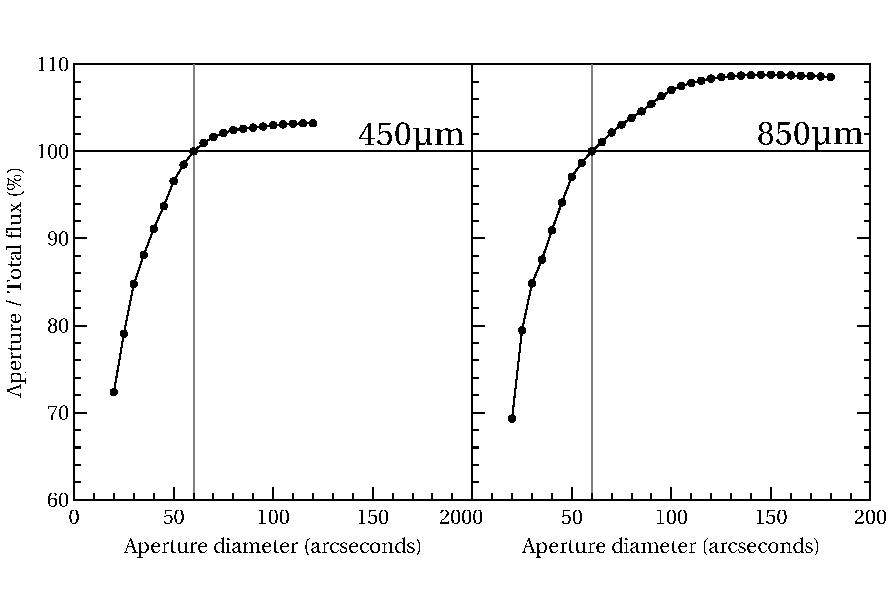
\includegraphics[width=0.95\linewidth]{curveofgrowth.eps}
\caption{\small Aperture photometry curve of growth normalised for a
60\arcsec\ aperture at 450$\mu$m \textbf{(left)} and 850$\mu$m \textbf{(right)}.
Figure taken from Dempsey et al. (2012).}
\label{fig:cog}
\end{figure}

\section{\xlabel{defconfig}dimmconfig.lis}
\label{app:dimm}
\begin{myquote}
\begin{verbatim}
# Number of iterations
#  positive number  = fixed number of iterations
#  negative number = max iterations if using chi^2 and/or map stopping criteria
numiter = -5

# Two convergence tests are available (used only if numiter is set to
# a negative value). They may be used simultaneously.
#
# chitol: threshold change in reduced chi^2 in subsequent iterations (requires
#         noi to be a component of modelorder). If there are any degeneracies
#         between model components (even if the map is reasonably constrained)
#         this is a bad test.
#
# maptop: threshold chance in the mean absolute difference between map pixels
#         in subsequent iterations, normalized by the estimated map RMS. This
#         is much more like a "by eye" test, that will stop the solution
#         when the map stops changing.

chitol = 1e-3
#maptol = 0.05

# method of estimating variance map
#  0 = propagate from the time-domain noise (requires noi model component)
#  1 = sample variance of data that land in each pixel
varmapmethod = 1

# Handle each subarray separately? Normally all data that were taken
# simultaneously at a given wavelength are handlded together.
#groupsubarray = 1

# If performing iterations in memory, maximum length (seconds) for concatenated
# data. If 0 attempt to concatenate entire continuous chunks.
maxlen = 0

# Model components/order (comma separated list in brackets)
# Note: components specified AFTER 'ast' will not be calculated for the
# first time until the second iteration.
#  dks = fit and remove dark squid for the column
#  com = remove common-mode signal
#  gai = if com specified, fit gain/offset of common mode
#  ext = apply extinction correction
#  ast = estimate the map and astronomical signal
#  flt = apply filter to time streams
#  noi = estimate time-domain variance
#  smo = time series smoothing using a median or mean boxcar filter
#  pln = remove plane from each time slice
#  tmp = remove externally define template such as azimuth

modelorder = (com,gai,ext,flt,ast,noi)

# Export model files as NDF?

# Specify a value of 1 or 0 to export all or none of the components
# You can also specify an array of components to export using the same
# format as modelorder. Note that you can specify additional
# components 'res' and 'qua' to what may be provided to modelorder if
# you wish to export the residual model or quality arrays
# respectively. Exportation of 'res' is implied if 'noi' is specified
# as it becomes the variance components of the resulting NDF for
# 'res'. 'qua' will become the quality component of any full 3-dimensional
# model (e.g. 'res', 'ast', 'flt', 'ext'), but no quality will be
# written to model components with different dimensions.

exportndf = 0
#exportndf = (com,gai,ast,flt,dks,smo,pln,tmp,res,noi,qua)

# Normally all data points in exported model components are set to BAD values
# wherever ther e is a bad bolometer established during map-making. Set
# this flag to prevent this behaviour.

#noexportsetbad = 1

# Export the logitude/latitude of every sample into a pair of NDFs?
# The file names will be the same as model components, except with
# sufficies equal to the AST "Symbol" attribute associated with the
# celestial axes ("ra"/"dec", "glon"/"glat", etc).

#exportlonlat = 1


# Create .MORE.SMURF.ITERMAPS extensions? If this parameter is set to
# a positive value, maps from each iteration and each chunk will be
# written.  If this is set to a negative value, only the final
# iteration will be written.
# itermap = 1


# Create .MORE.SMURF.BOLOMAPS single-beam map extensions?
#bolomap = 1

# Create .MORE.SMURF.SHORTMAPS extensions containing maps of every "shortmap"
# time slices? Alternatively, set to -1 to produce a map each time TCS_INDEX
# is incremented (i.e., each time a full pass through the scan pattern has
# been completed). Any other negative value is interpreted as a duration
# in seconds, and is converted to time slices using the (possibly
# down-sampled) sample frequency of the data being mapped.
#shortmap=-5.0  # This is 5 seconds, i.e. 1000 samples at 200 Hz sample rate

# Create .MORE.SMURF.FLAGMAPS extensions? To enable this feature set flagmap
# to an array containing a subset of the following bit flags. Each flagmap
# will then contain a count of the number of samples with a quality bit
# matching at least one of these flags, for each continuous chunk:
#
# BADDA   : flagged bad by the DA system
# *BADBOL : entire bolometer is turned off
# SPIKE   : flagged as a spike
# DCJUMP  : location of a DC level step
# STAT    : telescope was not moving within flagslow to flagfast
# COM     : portion of data did not match the common-mode
# FILT    : filtered data did not have sufficient contributions from good data
# NOISE   : bolometer was flagged as being too noisy in general
#
# *Note: If BADBOL is set the behaviour is slightly different than expected;
#        the bolometer will be completely ignored when creating the flag map.
#
# The flagmap is mostly useful to verify whether the spike, jump, and
# common-mode rejection is correlated with features in the map (e.g. bright
# sources), for all of the detectors that were used to produce the map, e.g.
#
#flagmap = (BADBOL,SPIKE,DCJUMP,COM)

# Create .MORE.SMURF.SAMPCUBES extensions providing data cubes of data samples
# that go into each map pixel?
#sampcube = 1

# Apply the flatfield if loading raw data? Default is 1 (true) -- you must
# explicitly set this to 0 if you want to produce a map in raw DAC units (and
# also supply raw data).

# ensureflat=0

# The gap (in time slices if positive and seconds if negative) between full
# calculations of the output map bolometer positions. Setting a larger value
# for this will speed up the map-maker but will introduce larger spatial
# errors. The default value of -0.5 (i.e. 100 samples at a sample rate of
# 200 Hz) seems to produce spatial errors of under 0.1 arc-sec. This
# level of errors seems to cause about 1% of bolometers samples to be
# pushed into a neighouring map pixel. For tstep=100, the calculation of
# bolometer positions speeds up by about a factor of 60. Setting tstep to
# 1 (or zero) causes all bolometer positions to be calculated in full,
# without any approximation.
#tstep = -0.5

# If the telescope is scanning slowly the data may be safely down-sampled
# to save memory and time. This parameter controls the minimum angular
# scale on the sky. The new sample frequency is chosen such that this
# scale will be preserved taking into account the average slew speed and
# the sample rate of the input files. If a positive value is selected, this
# gives the angular scale (in arcsec) to which the new sample rate will be
# matched. Alternatively, if a negative value is supplied, its magnitude will
# be multiplied by the PIXSIZE for the requested map. For example, the default
# here is to set it to -1 such that the time-series sample rate matches the
# pixel grid (in practice, a factor of 2 might make more sense as this would
# correspond to the Nyquist frequency of the map pixel grid).

#450.downsampscale = 2
#850.downsampscale = 4

downsampscale = -1

# Alternatively, if you wish to downsample to a specific sample rate it
# can be specified with downsampfreq in Hz.

# downsampfreq = 50.

# To test the response of the map-maker to different known
# astronomical sources, an external "fakemap" can be specified to
# provide an image of the sky that will produce additional
# astronomical signal to the time series. At present, the dimensions
# of this map must be identical to that of the real map. If the pixel
# ranges are not the same makemap will hault. A typical procedure may
# involve: (i) produce a map withe makemap; (ii) produce an image with
# simulated data with the same pixel dimensions; (iii) specify this
# new map for the "fakemap" parameter below. Note that this is a
# fully parsed ndf identifier, so you can do things like:
#
# fakemap = fakesky.sdf
# fakemap = fakesky[1:300,100:450]
#
# Additionally, you can specify a scalar scale factor, "fakescale", by
# which each pixel in the fakemap will be multiplied before adding to
# the data.
#
# fakescale = 23.5

# ----------------------------------------------------------------------------
# The following parameters control data-cleaning before iterations start
# ----------------------------------------------------------------------------

# set this to 0 to turn off all of the pre-mapmaking data cleaning

#doclean = 0

# Export the data immediately after data cleaning / before map-making?
# The file name will be the same as model components, except with the
# suffix "_cln". Even if doclean=0, the data will be exported immediately
# before map-making.

#exportclean = 1

# --- Mean subtraction is fairly useful ---

# subtract a baseline polynomial of this order
order = 1

# Use default apodisation based on filter frequency. This over-rides
# the default of zero in smurf_sc2clean.def. Keep the <undef> default
# for PAD which is set up in smurf_makemap.def.
apod = <undef>

# If zeropad is set, the padded regions are set to 0, and apodization
# is used to slowly roll-off the ends of the time series to 0. If zeropad
# is not set, a cubic is used to smoothly interpolate the end of the time
# series with the beginning (ensuring continuity in both the value and
# first derivative). In both cases, the purpose is to remove sharp edges
# that may cause ringing in the later FFT filtering steps. There are
# similar flags for DKS cleaning, and the FLT model.
#zeropad = 1

# --- badfrac ensures that bad data from DA system are ignored ---

# fraction of samples to be bad to flag entire bolo as dead
badfrac = 0.05


# --- flag data when we're moving either too slow or too fast ---

# Flag data taken while telescope was moving to slow such that sources
# are buried in 1/f noise, or too fast such that sources are smeared
# (value is a threshold slew velocity (arcsec/sec) measured in
# tracking coordinates). Assuming we would like to be able to sample
# scales of at least 30 arcsec (at least two 15 arcsec beams at 850),
# and assuming a typical 1/f knee of 1 Hz, the telescope needs to slew
# at least 30 arcsec/sec to place sources in the signal band above the
# knee. Also, assuming a sample rate of 200 Hz, we want to be able to
# fully sample the 450 and 850 beams. For now just set it to something
# that is bigger than we need, but be warned that point-sources may be
# smeared-out.

flagslow = 30
450.flagfast = 1000
850.flagfast = 1000

# --- Many of the following may not be useful ---

# If this flag is set, the common-mode calculation will be performed
# additionally as a pre-processing step. All parameters com.* and gai.*
# below are parsed and used (e.g., to also flag bad data and optionally
# flatfield off the relative response to the common-mode signal). If this
# pre-processing step is chosen, it is still possible to specify COM/GAI
# as model components in the iterative solution

#compreprocess=1

# An alternative to removing the simple common-mode is cleaning by way
# of principal component analysis (PCA). In this case, a new set of
# basis vectors (components) are calculated from the bolometer time-series
# such that they have 0 covariances. The amplitudes of these new correlated
# signals are then calculated, and the largest amplitude components can
# be removed. In this simplest case of white detectors noise + a common
# atmospheric signal, this operation would be similar to using compreprocess.
# However, PCA is capable of detecting multiple signals with different
# correlation patterns across the array.
#
# It is *ESSENTIAL* that the bolometer data first have their mean values
# removed (i.e., order=0), as this assumption is used to speed up the
# calculation.
#
# The main parameter for PCA cleaning is the threshold above
# which components will be removed from the bolometer time-series. For
# each component, the RMS amplitude across all bolometers is
# calculated -- a single positive number related to the average
# strength of the component. An iterative sigma clipper is then used
# to flag components that are more than thresh*RMS away from the mean value.
# This approach is quite arbitrary, but a value of about 4 seems reasonable
# for some test data. Be warned that this statistical black box will remove
# real correlated astronomical signals as well! As with common-mode removal,
# the actual impact on science will need to be calibrated with simulations.
# If this parameter is set to 0 no pca cleaning will occur.
#
# The other parameter is pcalen. Since the noise properties vary with time,
# pca cleaning seems to work better on shorter bits of data. pcalen specifies
# the chunk length that will be cleaned as a number of time slices (be
# careful if you have down-sampling turned on!). If set to 0 it will
# default to the length of the full time-series.

pcathresh = 0

# *** pcalen is currently buggy, don't use! ***
#pcalen = 0

# S/N threshold to detect DC steps. Note, this refers to the noise level
# in the bolometer data after it has been smoothed with a median filter of
# width given by DCSMOOTH. In order to find the equivalent threshold in
# the unsmoothed data, multiply the DCTHRESH value by # 1.25/sqrt(DCSMOOTH).
# For instance, the default values for DCSMOOTH (50) and DCTHRESH (25)
# correspond to a threshold of 25*1.25/sqrt(50) = 4.4 sigma in the
# unsmoothed data.
dcthresh = 25.0

# box size over which to fit data with a straight line on either side of
# a potential DC jump. If positive, in units of samples. If negative, in
# units of seconds.
dcfitbox = 30

# The maximum number of steps that can be corrected in each minute of
# good data (i.e. per 12000 samples) from a bolometer before the entire
# bolometer is flagged as bad. A value of zero will cause a bolometer to
# be rejected if any steps are found in the bolometer data stream.
dcmaxsteps = 10

#  If more than DCLIMCORR bolometer have a step at a given time, then all
#  bolometers are corrected for a step at that time, using lower thresholds.
#  Setting it to zero here switches off the correction of correlated
#  steps. Removing this line causes the default value of 10 to be used.
dclimcorr = 0

# The width of the median filter used to smooth a bolometer data stream
# prior to finding DC jumps. If positive, in units of samples. If negative,
# in units of seconds.
dcsmooth = 50

# S/N ratio to flag spikes with sigma-clipper
# spikethresh = 5

# Size of filter box for sigma-clipper, in units of samples if positive
# and seconds if negative.
# spikebox = 50

# Fill vicinity of spikes / DC steps with constrained realization of
# noise
fillgaps = 1

# The following filters are applied *before* the iterative loop. It is
# probably a better idea in general to do filtering with the 'flt'
# model component as described in the next section.

# Hard-edge high- and low-pass frequency-domain filter
#   e.g. keep only frequencies >= 0.1 Hz, and <= 90Hz

# filt_edgehigh = 0.1
# filt_edgelow = 90

# Alternatively, determine filter edges based on a range of requested
# spatial scales (arcsec), and using internal measurements of the
# average slew speed. These will override filt_edgehigh/filt_edgelow.
# For example, suppose the slew speed is 100 arcsec/sec. We want to
# ensure that the beam is fully sampled, say 2 arcsec at 450um. That
# scale is crossed in 2/100 = 0.02 s, so we don't need frequencies in
# the data above 1/0.02 = 50 Hz in this case (i.e. internally it will
# set filt_edgelow to 50Hz if filt_edge_smallscale is set to 2
# arcsec). Similarly, if we would like to attempt to preserve scales
# of 10 arcmin = 600 arcsec, we would want to keep frequencies that
# are greater than 1/(600/100.) = 0.17 Hz (i.e. setting
# filt_edge_largescale=600 would translate into filt_edgehigh = 0.17
# Hz).

# filt_edge_largescale = 600.
# 450.filt_edge_smallscale = 2.
# 850.filt_edge_smallscale = 4.

# Hard-edge band-cut frequency-domain notch filters.
# filt_notchlow gives lower edges of frequencies to cut in Hz
# filt_notchhigh gives upper edges of frequencies to cut in Hz
#   e.g. remove 25--35 Hz  and 55--65 Hz
#filt_notchlow  = (25,55)
#filt_notchhigh = (35,65)

# Should a whitening filter be applied to compensate for 1/f noise?
# whiten = 1

# Clip bolometers based on their noise. This step will remove any
# bolometers noisier than noisecliphigh standard deviations above the
# median, or noisecliplow standard deviations below the
# median. Normally the noise clipping happens at the end of the
# cleaning stage, but if you set noiseclipprecom it will instead occur
# immediately prior to common-mode subtraction (see comppreprocess)
noisecliphigh = 4.0
#noisecliplow = 4.0
#noiseclipprecom = 1

# ----------------------------------------------------------------------------
# A number of analagous parameters to clean dark squid signals before fitting
# them to the data (only relevant if DKS is specified as a model component).
# Note that if padding has been added to the bolometer data, it is
# automatically added to the dark squids as well (i.e. there is no
# cleandk.padstart/padend).
# ----------------------------------------------------------------------------

cleandk.apod=<undef>
cleandk.badfrac = 0.05
cleandk.dcfitbox = 30
cleandk.dcmaxsteps = 10
cleandk.dcthresh = 25.0
cleandk.dcsmooth = 50
cleandk.fillgaps = 1
#cleandk.filt_edgelow = 0
#cleandk.filt_edgehigh = 0
#cleandk.filt_notchlow = <undef>
#cleandk.filt_notchhigh = <undef>
#cleandk.noisecliphigh = 0.0
#cleandk.noisecliplow = 0.0
#cleandk.noiseclipprecom = 0
#cleandk.whiten = 0
cleandk.order = 1
#cleandk.spikethresh = 0
#cleandk.spikebox = 50
#cleandk.zeropad = 1

# ----------------------------------------------------------------------------
# These parameters control the iterative model components
# ----------------------------------------------------------------------------


#  Set this flag to a non-zero value to use the old COM algorithm that was
#  used up to 15-MAY-2012. The new algorithm in general provides faster
#  and smoother convergence.
com.oldalg = 0

#  Set this flag to calculate a separate common-mode signal for each
#  subarray. If not set, a single common-mode signal will be calculated from
#  all subarrays at a given wavelength simultaneously.
#com.perarray = 1

#  The new COM algorithm uses the sigma-clipped weighted mean of all
#  bolometer values at each time slice as the common-mode signal. The
#  following parameters control the sigma-clipping algorithm.
#
#  The number of n-sigma clipping iterations (1 => no clipping)
com.niter = 1

#  The number of standard deviations at which the n-sigma clipping
#  algorithm clips.
com.nsigma = 3

# delay calculation of COM until after the first iteration? (good if
# the astronomical signal is expected to dominate the sky signal)
#com.notfirst = 1  (can only be used with the old COM algorithm)

# If this flag is set, the common-mode will be estimated while
# iteratively flagging and removing outlier detectors as
# usual. However, once the flagging is completed, the common-mode will
# not actually be removed from the time-series (and if the model is
# exported, it will be set to 0).
#com.noremove=1   (can only be used with the old COM algorithm)

# low-pass boxcarfilter on COM (samples) to assist with convergence
# if boxfact set reduce width of boxcar by this factor each iteration
# boxmin specifies a minimum width below which it can't be reduced.
# Positive values for com.boxcar are interpreted as a number of samples,
# and negative values as a number of seconds (converted to samples using
# the downsampled sample rate).
#com.boxcar = 10   (can only be used with the old COM algorithm)
#com.boxcar  = 400
#com.boxfact = 0.5
#com.boxmin  = 10

# the following COM parameters control the rejection of bad detectors
# based on the gain and correlation coefficients for the fit of the
# common-mode signal to each detector (good at identifying bolo signals
# with bizarre gains, or shapes if they have for example steps in them). These
# are basically sigma-clippers; outliers are removed at the given threshold
# and then new means and sample standard deviations are measured until
# convergence. The time axis is divided up into one or more equal sized boxes,
# and a separate fit is performed for each box. If you wish to completely
# disable the flagging of outlier bolometers compared with the common-mode,
# simply set com.noflag=1
#
# com.noflag: if set, disable flagging of bad bolos using common-mode
# com.gain_box: the number of time slices (or seconds if negative) in a box
# com.corr_tol: n-sigma away from mean correlation coefficient tolerance
# com.corr_abstol: the absolute lower limit of acceptable correlation
# com.gain_tol: n-sigma away from mean gain coefficient tolerance
# com.gain_abstol: absolute factor away from mean gain coefficient tolerance
# com.gain_fgood: minimum fraction of good boxes for a usable bolometer
# com.gain_rat: ratio of largest usable gain to mean gain for a bolometer

com.noflag = 0
com.corr_tol = 5
com.gain_tol = 5
com.gain_abstol = 3

# by default negative gains are used to flag bad bolometer data. However, if
# this parameter is set to 0 negative values will be allowed
#com.gain_positive = 0

# Do not set com.gain_box lower than about 6000 (or -30) which corresponds to
# 30s, or roughly the fridge oscillation period.
com.gain_box = -30.0
#com.corr_abstol = 0.2
#com.gain_fgood = 0.25
#com.gain_rat = 4.0

# low-pass filter dark squid signals using boxcar of this width (if dks
# model is specified). Value is in samples (after any downsampling) if
# positive and seconds if negative.
dks.boxcar = 100

# if set, replace dead dark squids with average of working dark squids
dks.replacebad = 0

# do we want to calculate noise weights immediately after pre-conditioning,
# or wait until we have the first iteration of the residual? The former can
# reduce execution time if noiseclip is also set since both operations
# share a single FFT.
#noi.calcfirst = 1

#  Determines the number of time slices used to determine the noise level
#  in a section of a bolometer time stream. If zero, then the whole bolometer
#  time stream is used, and each bolometer has only one variance value. If
#  non-zero, each bolometer time stream is divided up into boxes
#  containing the specified number of time slices, and a separate variance
#  is found for each box. This variance is then used for each sample in the
#  box, so each bolometer ends up with a variance for every time slice.
#  Negative values are interpreted as number of seconds, and positive values
#  as a number of down-sampled time slices. The default is zero.
#  noi.box_size = -30.0

# additional despiking / DC step finding after each iteration within noi
# calculation. Setting noi.spikebox to 50 will check for excursions
# from a rolling median filter in a box of length 50 samples (negative
# values are interpreted as seconds and converted to samples using the
# downsampled sample rate).
#noi.spikethresh = 10
#noi.spikebox = 50
noi.fillgaps = 1

# explicitly turn off iterative DC step finding for now
noi.dcfitbox = 0

#  Use default apodisation based on filter frequency
flt.apod = <undef>

# iterative filter.
#450.flt.filt_edgehigh = 0.1
#850.flt.filt_edgehigh = 0.3
#flt.filt_edgelow = 90
#flt.filt_notchlow  = (25,55)
#flt.filt_notchhigh = (35,65)
#flt.zeropad = 1

450.flt.filt_edge_largescale=600
850.flt.filt_edge_largescale=300

# delay calculation of FLT until after the first iteration? May help
# with negative structure around bright sources

#flt.notfirst = 1

# extinction correction (see EXTINCTION task for further information)
# Best is to use WVM, uses continuously varying measurements as a
# function of time stored with each observation. This is the default if
# nothing is specified.
#
# tausrc   : auto, wvmraw, csotau, filtertau
# taumethod: adaptive, full, quick

# filtertau "tausrc" requires a filtertau entry
# csotau is optional for "auto" and "csotau" tausrc. If not provided
# the value will be calculated from the header.

# csotau   : use value only if tausrc=csotau
# filtertau: use only if tausrc=filtertau

ext.tausrc    =auto
ext.taumethod =adaptive
#ext.csotau    = 0.2
#ext.filtertau = 0.2

# Use the GAIn/COMmon mode to re-calculate the flatfield? Probably a
# good idea in most cases, but dangerous for short scans of very bright
# sources because the astronomical signal may completely dominate
# sky signal.

#gai.flatfield = 1 (can only be used with the old COM algorithm)

# Large-scale degenerate structures can grow in the maps with iterations and
# so some constraints are required.
#
# One method is to use an FFT-base high-pass filter after each
# iteration.  Using ast.gaussbg will effectively smooth the map with a
# Gaussian of the supplied FWHM and subtract this background from the
# map after each iteration.  This has the nice property that it is a
# fairly easily understood linear filtering operation.
#
# Another method is to constrain regions of the map to 0.
#
# If ast.zero_mask is set, the reference image, as indicated by the
# makemap ADAM parameter REF, will be interpreted as containing a
# user-defined mask. Using the REF image ensures that the mask and the
# output image of MAKEMAP are on the same pixel grid. The pixels in
# the map that are to be constrained to 0 should be set to the bad
# value. All other pixels will be allowed to vary during map-making.
#
# Using ast.zero_lowhits will set a threshold region where
# the hits are this fraction lower than the mean.
#
# Using ast.zero_circle defines a circle on the map outside of which
# the map will be constrained to zero. The 3 parameters are:
# Longitude, Latitude, Radius of the circle, in decimal degrees, in
# the coordinate system of the map (e.g., RA and Dec.). Alternatively
# a single parameter may be given (the radius), and then the centre
# of the circle will default to the reference coordinates for the
# centre of the map (e.g. the tangent point).
#
# The ast.zero_snr parameter will create a mask based on map SNR. For
# example, if it is set to 5, after each iteration all pixels with a
# SNR below this threshold will be set to 1 (other pixels are left at zero).
# Each contiguous clump of zero-valued pixels (i.e. "source" pixels) in
# this basic mask can then be expanded to encompass adjacent pixels that
# are above a second, lower, SNR threshold given by ast.zero_snrlo. So
# for instance, setting ast.zero_snrlo to 1 will cause the basic mask
# thresholded at SNR = 5 to be expanded down to an SNR of 1. This dual
# thresholding system prevents noise spikes above the lower threshold being
# interpreted as source pixels.
#
# The ast.zero_snr_fwhm parameter gives the FWHM of a Gaussian (in arcsec)
# with which to smooth the final mask produced as a consequence of setting
# the ast.zero_snr value. If it is set to zero, no smoothing is performed.
# The smoothing occurs once all chunks of the map have converged, and a new
# map is then created using the smoothed mask as if it had been supplied via
# "ast.zero_mask". Consequently, setting ast.zero_snr_fwhm causes the time
# taken to create the final map to nearly double.
#
# The ast.zero_snr_low parameter gives the value (in the range 0.0 to 1.0)
# at which to threshold the smoothed mask specified by ast.zero_snr_fwhm.
# If it is negative, the value is taken as the max smoothed value of a blob
# containing "ast.zero_snr_low" pixels. Thus a value of "-1.1" will cut at
# a height just sufficient to remove blobs of a single pixel form the mask.
# A value of "-2.1" would remove blobs of two pixels form the mask, etc.
#
# If ast.zero_niter is set, it gives the number of iterations for which
# the AST model should be masked. The default is zero, which means "mask
# on all iterations". However, if ast.zero_notlast is set, the mask will
# will not be applied on the last iteration, even if ast.zero_niter is zero.
# This feature will probably be useful for deep point-source observations
# for which the large-scale noise is not as important, but keeping as much
# data around the edges of the map is.

#ast.gaussbg = 120
#ast.zero_mask = 1
#ast.zero_circle = (70.72333,36.115,0.0083333)
#ast.zero_lowhits = 0.1
#ast.zero_notlast = 1
#ast.zero_snr = 5
#ast.zero_snrlo = 1
#ast.zero_snr_fwhm = 60
#ast.zero_snr_low = -1.1

# The common-mode can also be masked to exclude known source areas
# from the common-mode estimation. The zero of parameters are directly
# analogous to those for applying a zero constraint to the map. The only
# difference is that the zero_snr and zero_lowhits constraints will be
# ignored on the first iteration since they require an estimate of the map
# to be available.
#com.zero_mask = 1
#com.zero_circle = (70.72333,36.115,0.0083333)
#com.zero_lowhits = 0.1
#com.zero_notlast = 1
#com.zero_snr = 5
#com.zero_snrlo = 1

# The FLT model can also be masked to exclude known source areas. This can
# reduce the number of iterations needed for convergence, and may also
# reduce the noise in the final map, and reduce ringing and "bowls" around
# bright sources. The parameters are directly analogous to those for applying
# a zero constraint to the map. The only difference is that the zero_snr and
# zero_lowhits constriants will be ignored on the first iteration since they
# require an estimate of the map to be available. Note
#flt.zero_mask = 1
#flt.zero_circle = (70.72333,36.115,0.0083333)
#flt.zero_lowhits = 0.1
#flt.zero_notlast = 1
#flt.zero_snr = 5
#flt.zero_snrlo = 1
flt.zero_niter = 2

# The AST model can also perform map-based de-spiking after the first
# iteration provided that there is also a NOI model present. The value
# of ast.mapspike indicates a SNR threshold sigma-clip based on the
# scatter of the samples that contribute to a given pixel value about
# the map value.
ast.mapspike = 10

# Smooth the time series

# don't smooth on the first iteration
smo.notfirst = 1

# Type of filter: mean or median
smo.type = median

# width of smoothing box (roughly equivalent to FLT with a high-pass
# filter at cutoff frequencies 0.1 and 0.3 Hz for 450 and 850
# respectively). If positive, value is in samples. If negative, value is
# in seconds.
450.smo.boxcar = -10
850.smo.boxcar = -3

# The TMP model fits an externally defined template to each bolometer
# time-series. The only parameter defines what that template
# is. Presently the only two valid options are "state_az" and
# "state_el" to use the telescope azimuth and elevation
# respectively. The former seems to be a good way for removing
# magnetic field pickup. You may also request that the sine or or
# cosine be taken of the template before fitting (tmp.dosin and
# tmp.docos respectively), and before doing that a fixed offset may
# be added (tmp.trigoffset). It is assumed that the template
# quantities are in radians.
#
# tmp.source = state_az
# tmp.dosin = 1
# tmp.trigoffset = 0

\end{verbatim}
\end{myquote}


\section{\xlabel{special}Specialised Configuration Files}
\label{app:special}

\subsection{dimmconfig\_bright\_extended.lis}
\begin{myquote}
\begin{verbatim}
^$STARLINK_DIR/share/smurf/dimmconfig_bright.lis

# *** Specialized config for scans of bright/extended structure ***
#
# For bright extended regions we turn on zero-masking based on a map
# pixel SNR threshold of 5-sigma. This prefents ringing a round bright
# sources, but will completely flatten the map in low-SNR regions.
#
# ****************************************************************

# these set up map-based convergence tests: a maximum of 40 iterations,
# but it will stop if there is a mean absolute change in the map between
# subsequent iterations of less than 5% (note also that we explicitly
# turn the chi^2 test off).

numiter=-40
chitol=<undef>
maptol=0.05

ast.zero_notlast = 1
ast.zero_snr = 5
\end{verbatim}
\end{myquote}

\subsection{dimmconfig\_bright\_compact.lis}
\begin{myquote}
\begin{verbatim}
^$STARLINK_DIR/share/smurf/dimmconfig_bright.lis

# *** Specialized config for bright, isolated compact sources ***
#
# This config file is for maps with a bright central compact source. In
# particular the strategy is aimed at short scans of calibrators (which
# may be quite bright).
#
# We constrain the map using ast.zero_circle=(0.01666), which sets all
# pixels beyond 60 arcsec to zero until the last iteration.  A word of
# warning: if the source is near the edge of the map (or has an extent
# large than the size of this mask!) this configuration may give odd
# results due to the value of ast.zero_lowhits!  If you suspect a
# problem, compare the location of the source with the zero-masked
# pixels (see QUALITY component of the resulting map). If the mask
# overlaps with the source, try modifying the radius.
#
# ***********************************************************

# these set up map-based convergence tests: a maximum of 40 iterations,
# but it will stop if there is a mean absolute change in the map between
# subsequent iterations of less than 5% (note also that we explicitly
# turn the chi^2 test off).

numiter=-40
chitol=<undef>
maptol=0.05

# use boundary constraints since the source is assumed to be isolated
ast.zero_circle = (0.0166666666)
ast.zero_notlast = 1

#  Mask the data when forming th FLT model in order to exclude the
#  source, but only on the first two iterations. This usually speeds up
#  convergence.
flt.zero_circle = (0.0166666666)
flt.zero_niter = 2

# Per array common-mode should be fine here since we are dealing with
# a compact source. It seems to make things more stable.
com.perarray = 1

# we can get away with harsher filtering since the boundary conditions are
# quite tight
450.flt.filt_edge_largescale=200
850.flt.filt_edge_largescale=200
\end{verbatim}
\end{myquote}

\subsection{dimmconfig\_blank\_field.lis}
\begin{myquote}
\begin{verbatim}
^$STARLINK_DIR/share/smurf/dimmconfig.lis

# *** Specialized config for deep scans of blank fields ***
#
# This config is aimed primarily at reducing blank fields -- extremely
# deep observations for detecting the individual point sources that
# produce the cosmic infrared background.
#
# Since there are no bright objects, a single high-pass filter is
# applied at the start, and no other iterative filtering is
# performed. A harsher high-pass filter is applied than in the default
# configuration since no appreciable large-scale structure is
# expected.
#
# When reducing a large data set it might be useful to write out the
# maps from each iteration/chunk by setting itermap=1.  This will
# produce a series of extensions (.MORE.SMURF.ITERMAPS) for each
# iteration, and for each continuous chunk of data. For example, they
# can be viewed using:
#
#   gaia [output map name].more.smurf.itermaps
#
# By flipping through the more.smurf.itermaps extension it is possible
# to get a good feel for how well the map is converging (and whether
# you would like more or less iterations). It is also useful to
# identify particularly noisy portions of the data. If the last
# iteration of a given chunk looks poor compared with the other chunks,
# you can identify the input files from the FITS header of the
# extension, and remove them.
#
# If you only want to see a single itermap written for the final iteration
# of each chunk set itermap=-1
#
# Setting shortmap=1 will give similar information, except now writing
# out a map each time a single time around the scan pattern has been
# completed (only for the final iteration).
#
# ***********************************************************

numiter = 4

modelorder = (com,ext,ast,noi)

# Use time-domain spiker first because we are only doing a single FFT-based
# high-pass filter before the iterations start.

spikethresh = 10
spikebox = 50

# Heavier high-pass filtering. Note that the default padding/apodization
# that will be used is the number of samples that corresponds to the
# period of the knee frequency in the high-pass filter (i.e. 200*(1/freq) )

450.filt_edge_largescale = 200
850.filt_edge_largescale = 200

# Large-scale structure is not an issue so treat each subarray independently
# for common-mode removal
com.perarray = 1
\end{verbatim}
\end{myquote}


\subsection{dimmconfig\_bright.lis}

This file is included as although it is not used in its own right it
form the basis (on top of \texttt{dimmconfig.lis} for both
\texttt{dimmconfig\_bright\_compact.lis} and
\texttt{dimmconfig\_bright\_extended.lis}
\begin{myquote}
\begin{verbatim}
^$STARLINK_DIR/share/smurf/dimmconfig.lis

# *** Specialized config for bright sources ***
#
# Maps of bright sources, regardless of their physical extent,
# generally require less aggressive rejection of bad data due to the
# presence of strong astronomical signals (which may accidentally be
# identified as steps, throw-off the common-mode bolometer rejection,
# contaminate noise estimates etc.). They also generally require a
# larger number of iterations to maximize the sensitivty to large
# dynamic signal ranges in the map.
#
# ***********************************************************

numiter = 20

# Much weaker bolometer noise clip
noisecliphigh = 10.0

# Less aggressive DC step finder to avoid problems with bright sources
dcthresh = 100

# Less aggressive bolo flagging. Also, handle bolos in entire
# chunks. Even if we get chunked common-mode flagging to work much
# better, these maps of bright point sources may cause problems.

com.corr_tol = 7
com.gain_tol = 7
com.gain_abstol = 5
#com.gain_box = 600000
\end{verbatim}
\end{myquote}

\section{\xlabel{acronyms}List of Acronyms}

\begin{description}

\item[CSO]\quad Caltech Submillimetre Observatory

\item[DIMM]\quad Dynamic Iterative Map-Maker

\item[FCF]\quad Flux Conversion Factor

\item[FWHM]\quad Full-Width at Half-Maximum

\item[GAIA]\quad Graphical Astronomy and Image Analysis Tool

\item[JCMT]\quad James Clerk Maxwell Telescope

\item[NEFD]\quad Noise Equivalent Flux Density

\item[PSF]\quad Point Spread Function

\item[S2SRO]\quad SCUBA-2 Shared Risk Observing which took place in
  February and March 2010.

\item[SCUBA]\quad Submillimetre Common User Bolometer Array

\item[SCUBA-2]\quad Submillimetre Common User Bolometer Array-2

\item[SMURF]\quad Sub-Millimetre User Reduction Facility

\item[S/N]\quad Signal-to-Noise ratio

\item[WVM]\quad Water Vapour radioMeter


\end{description}

\end{document}


